\documentclass[english]{article}
\usepackage{graphicx}
\usepackage{amsmath}
\usepackage{hyperref}
\usepackage{setspace}
\usepackage{apacite}
\usepackage{hyperref}
\usepackage[sort]{natbib}
\usepackage{pxfonts}
\usepackage[utf8]{inputenc}
\usepackage[left=1in,right=1in,top=1in,bottom=1in]{geometry}
\usepackage[left]{lineno}
\usepackage{soul}
\linenumbers

%\newcommand{\ttests}{S1}
\newcommand{\intact}{S1}
\newcommand{\para}{S2}
\newcommand{\word}{S3}
\newcommand{\rest}{S4}

\title{High-level cognition during story listening is reflected in
  high-order dynamic correlations in neural activity patterns}

\author{Lucy L. W. Owen$^1$, Thomas H. Chang$^{1,2}$, and\
  Jeremy R. Manning\textsuperscript{$1, \dagger$}\\
  [0.1in]$^1$Department of Psychological and Brain
  Sciences,\\Dartmouth
  College, Hanover, NH\\
  $^2$Amazon.com, Seattle, WA\\
  \textsuperscript{$\dagger$}Address correspondence to
  jeremy.r.manning@dartmouth.edu}


\begin{document}
\maketitle


\begin{abstract}
  Our thoughts arise from coordinated patterns of interactions between
  brain structures that change with our ongoing experiences.
  High-order dynamic correlations in neural activity patterns reflect
  different subgraphs of the brain's connectome that display
  homologous lower-level dynamic correlations.  We tested the
  hypothesis that high-level cognition is supported by high-order
  dynamic correlations in brain activity patterns.  We developed an
  approach to estimating high-order dynamic correlations in timeseries
  data, and we applied the approach to neuroimaging data collected as
  human participants either listened to a ten-minute story, listened
  to a temporally scrambled version of the story, or underwent a
  resting state scan.  We trained across-participant pattern
  classifiers to decode (in held-out data) when in the session each
  neural activity snapshot was collected.  We found that classifiers
  trained to decode from high-order dynamic correlations yielded the
  best performance on data collected as participants listened to the
  (unscrambled) story.  By contrast, classifiers trained to decode
  data from scrambled versions of the story or during the resting
  state scan yielded the best performance when they were trained using
  first-order dynamic correlations or non-correlational activity patterns.  We
  suggest that as our thoughts become more complex, they are supported
  by higher-order patterns of dynamic network interactions throughout
  the brain.
\end{abstract}

\doublespacing

\section*{Introduction}
A central goal in cognitive neuroscience is to elucidate the
\textit{neural code}: the mapping between (a) mental states or
cognitive representations and (b) neural activity patterns. One means
of testing models of the neural code is to ask how accurately that
model is able to ``translate'' neural activity patterns into known (or
hypothesized) mental states or cognitive
representations~\citep[e.g.,][]{HaxbEtal01, NormEtal06, TongPrat12,
  MitcEtal08a, KamiTong05, NishEtal11, PereEtal18, HuthEtal12,
  HuthEtal16}.  Training decoding models on different types of neural
features (Fig.~\ref{fig:patterns}a) can also help to elucidate which
specific aspects of neural activity patterns are informative about
cognition-- and, by extension, which types of neural activity patterns
might comprise the neural code.  For example, prior work has used
region of interest analyses to estimate the anatomical locations of
specific neural representations~\citep[e.g.,][]{EtzeEtal09}, or to
compare the relative contributions to the neural code of multivariate
activity patterns versus patterns of dynamic correlations between
neural activity patterns~\citep[e.g.,][]{MannEtal18, FongEtal19}.  An
emerging theme in this literature is that cognition is mediated by
dynamic interactions between brain structures~\citep{SporHone06,
  BassEtal06, Turk13, DemeEtal19, SoloEtal19, LuriEtal18, PretEtal17,
  ZouEtal19, MackEtal17}.


\begin{figure}[tp]
  \centering
  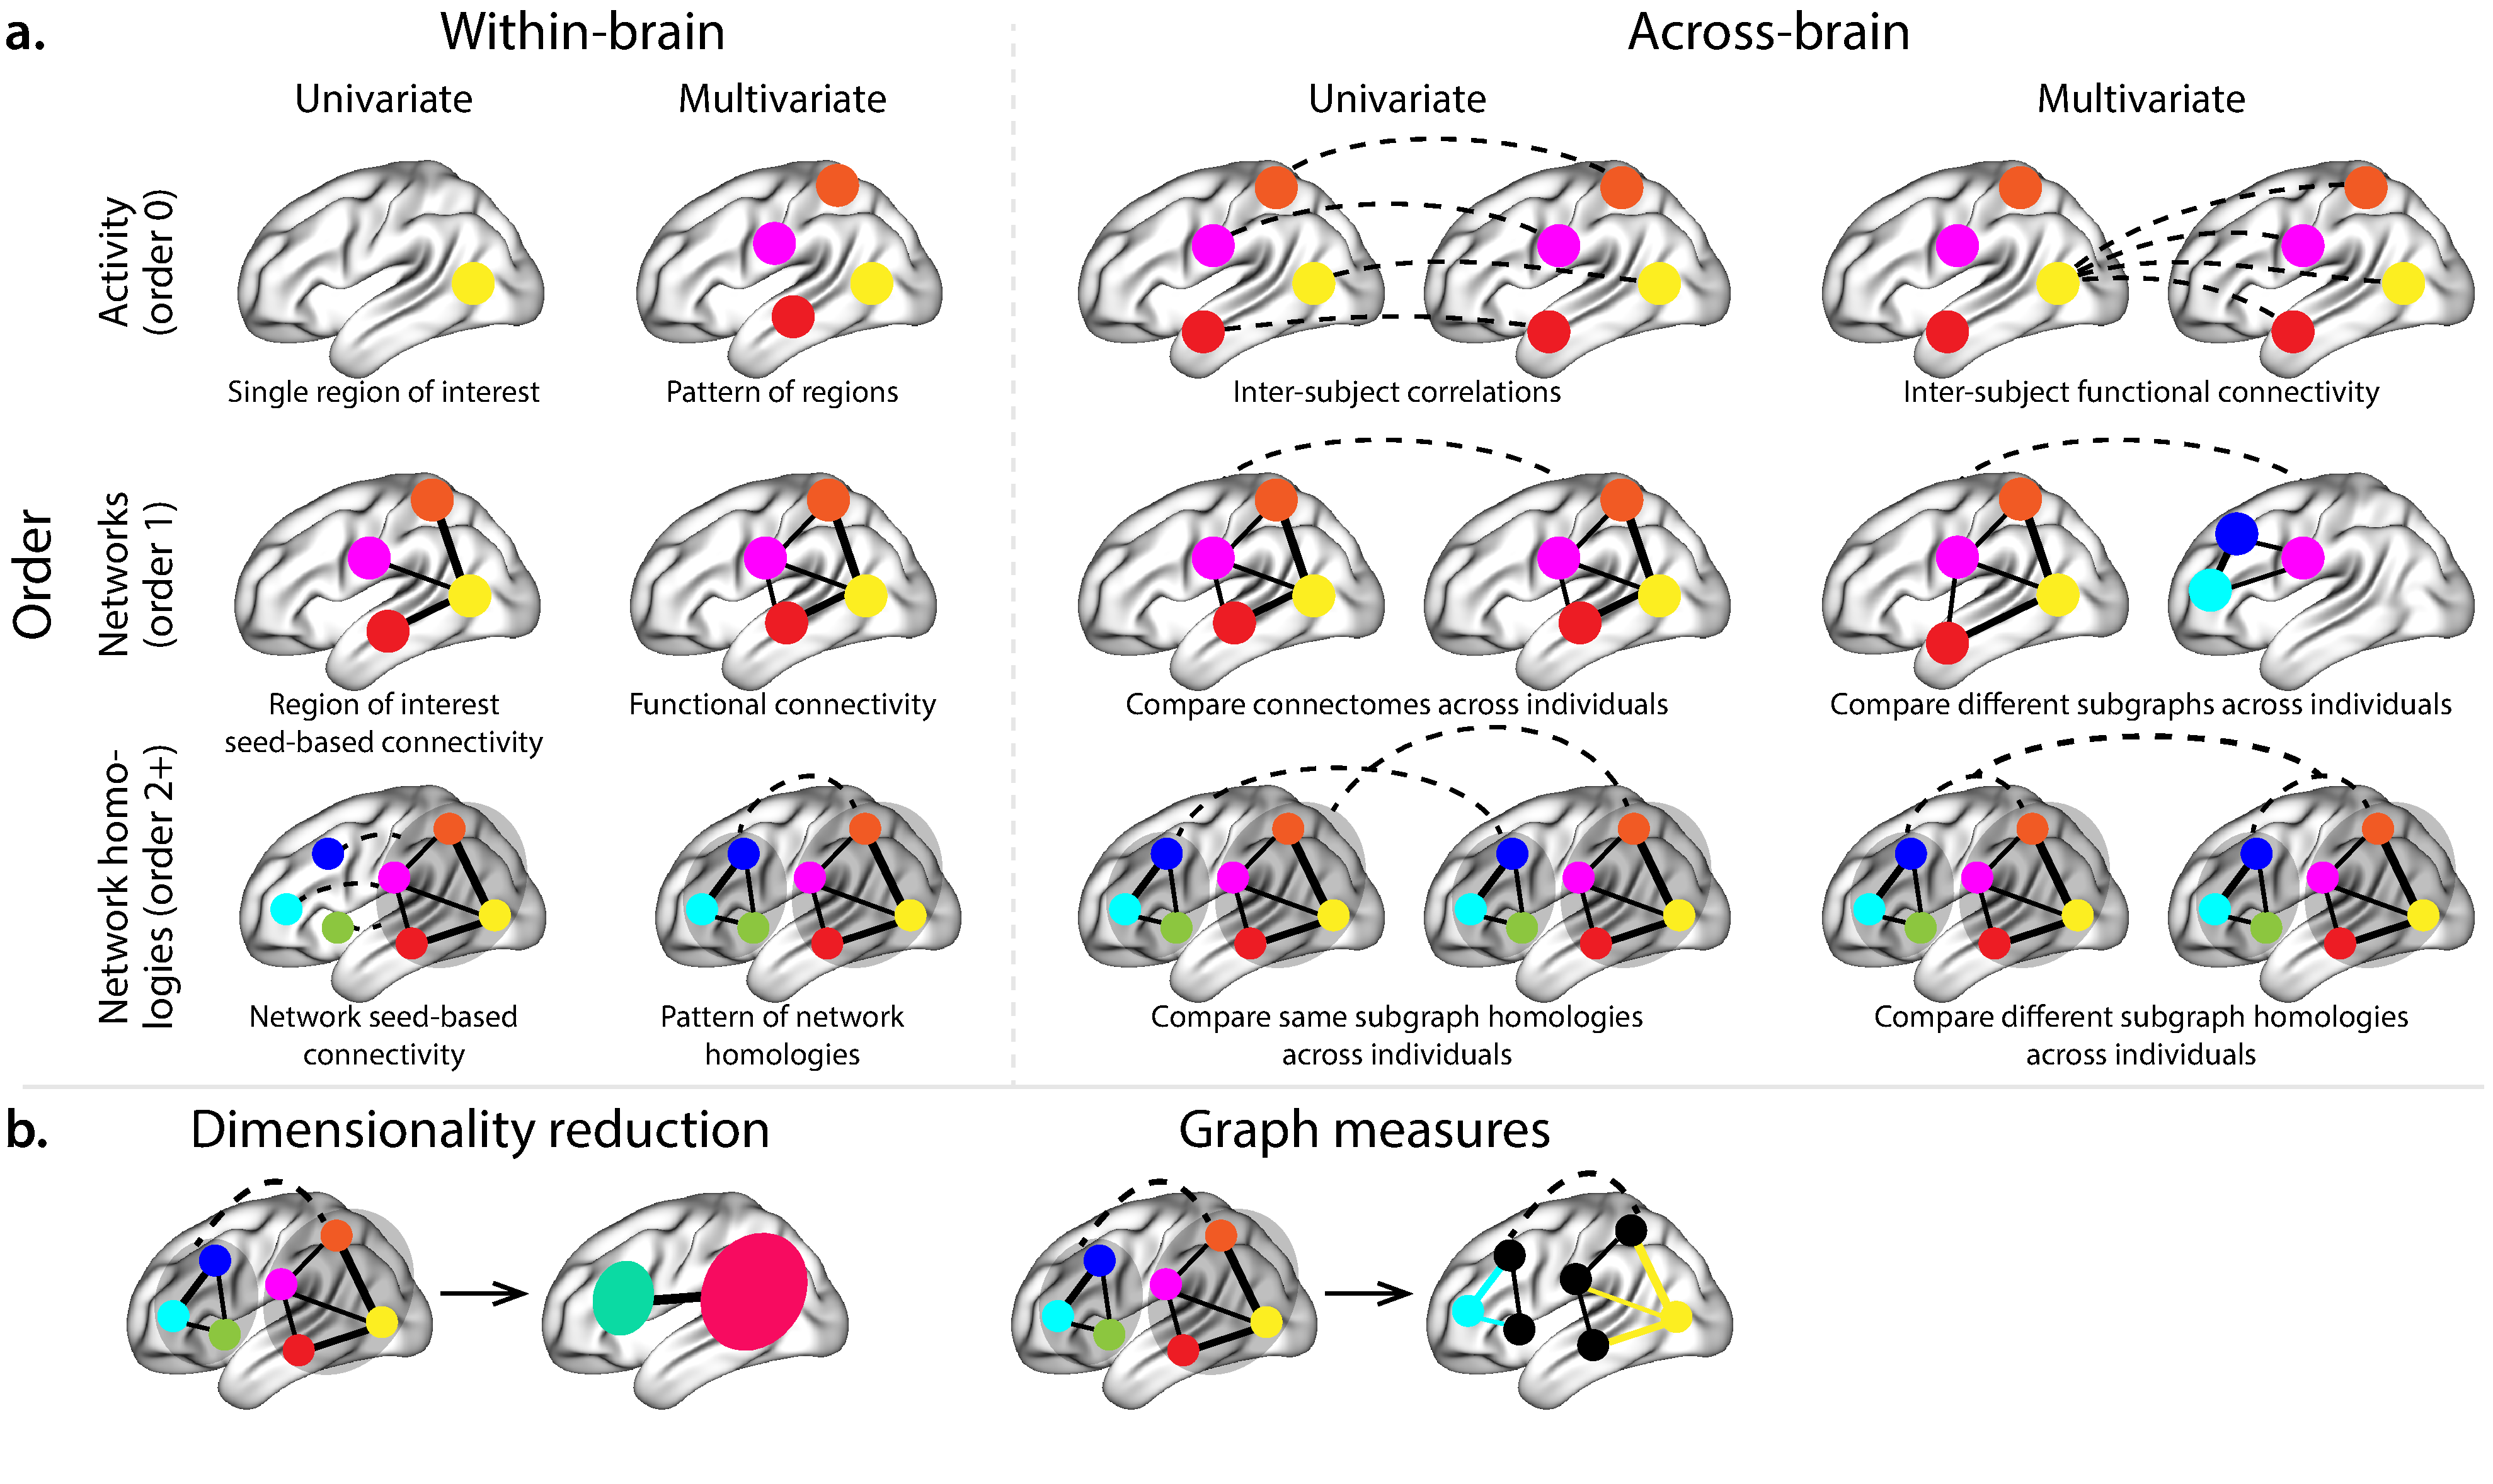
\includegraphics[width=\textwidth]{figs/patterns}
  \caption{\textbf{Neural patterns.  a. A space of neural analyses}
    Within-brain analyses are carried out within a single brain,
    whereas across-brain analyses compare neural patterns across two
    or more individuals' brains.  Univariate analyses characterize the
    activities of individual units (e.g., nodes, small networks,
    hierarchies of networks, etc.), whereas multivariate analyses
    characterize the patterns of activities across units.  Order 0
    patterns involve individual nodes; order 1 patterns involve
    node-node interactions; order 2 (and higher) patterns relate to
    interactions between homologous networks.  Each of these patterns
    may be static (e.g., averaging over time) or dynamic.
    \textbf{b. Summarizing neural patterns.}  To efficiently compute
    with complex neural patterns, it can be useful to characterize the
    patterns using summary measures.  Dimensionality reduction
    algorithms project the patterns onto lower-dimensional spaces
    whose dimensions reflect weighted combinations of the dimensions
    in the original space.  Graph measures characterize each unit's
    participation in its associated network.}
  \label{fig:patterns}
\end{figure}

Studies of the neural code to date have primarily focused on
univariate or multivariate neural patterns~\citep[for review
see][]{NormEtal06}, or (more recently) on patterns of dynamic
first-order correlations~\citep[i.e., interactions between pairs of
brain structures;][]{MannEtal18, FongEtal19, LuriEtal18, PretEtal17,
  ZouEtal19, DemeEtal19}.  We wondered what the future of this line of
work might hold.  For example, is the neural code mediated by
higher-order interactions between brain structures~\citep[e.g.,
see][]{ReimEtal17}?  Second-order correlations reflect
\textit{homologous} patterns of correlation.  In other words, if the
dynamic patterns of correlations between two regions, $A$ and $B$, are
similar to those between two other regions, $C$ and $D$, this would be
reflected in the second-order correlations between ($A$--$B$) and
($C$--$D$).  In this way, second-order correlations identify
similarities and differences between subgraphs of the brain's
connectome.  Analogously, third-order correlations reflect homologies
between second-order correlations-- i.e., homologous patterns of
homologous interactions between brain regions.  More generally,
higher-order correlations reflect homologies between patterns of
lower-order correlations.  We can then ask: which ``orders'' of
interaction are most reflective of high-level cognitive processes?

Another central question pertains to the extent to which the neural
code is carried by activity patterns that directly reflect ongoing
cognition~\citep[e.g., following][]{HaxbEtal01, NormEtal06}, versus
the dynamic properties of the network structure itself, independent of
specific activity patterns in any given set of regions~\citep[e.g.,
following][]{BassEtal06}.  For example, graph measures such as
centrality and degree~\citep{BullSpor09} may be used to estimate how a
given brain structure is ``communicating'' with other structures,
independently of the specific neural representations carried by those
structures.  If one considers a brain region's position in the network
(e.g., its eigenvector centrality) as a dynamic property, one can
compare how the positions of different regions are correlated, and/or
how those patterns of correlations change over time.  We can also
compute higher-order patterns in these correlations to characterize
homologous subgraphs in the connectome that display similar changes in
their constituent brain structures' interactions with the rest of the
brain.

To gain insights into the above aspects of the neural code, we
developed a computational framework for estimating dynamic high-order
correlations in timeseries data. This framework provides an important
advance, in that it enables us to examine patterns of higher-order
correlations that are computationally intractable to estimate via
conventional methods.  Given a multivariate timeseries, our framework
provides timepoint-by-timepoint estimates of the first-order
correlations, second-order correlations, and so on.  Our approach
combines a kernel-based method for computing dynamic correlations in
timeseries data with a dimensionality reduction step
(Fig.~\ref{fig:patterns}b) that projects the resulting dynamic
correlations into a low-dimensional space.  We explored two
dimensionality reduction approaches: principle components
analysis~\citep[PCA;][]{Pear01}, which preserves an approximately
invertible transformation back to the original data~\citep[e.g., this
follows related approaches taken by][]{McInJirs19, TokeSomm19,
  GonzEtal19}; and a second non-invertible algorithm that explored
patterns in eigenvector centrality~\citep{Land95}.  This latter
approach characterizes correlations between each feature dimension's
relative \textit{position} in the network in favor of the specific
activity histories of different features~\citep[also
see][]{BetzEtal19, SizeEtal18, ReimEtal17}.

We validated our approach using synthetic data where the underlying
correlations were known.  We then applied our framework to a
neuroimaging dataset collected as participants listened to either an
audio recording of a ten-minute story, listened to a temporally scrambled
version of the story, or underwent a resting state
scan~\citep{SimoEtal16}.  We used a subset of the data to train
across-participant classifiers to decode listening times using a blend
of neural features (comprising neural activity patterns, as well as
different orders of dynamic correlations between those patterns that
were inferred using our computational framework).  We found that both
the PCA-based and eigenvector centrality-based approaches yielded
neural patterns that could be used to decode accurately (i.e., well above
chance).  Both approaches also yielded the best decoding accuracy for
data collected during (intact) story listening when high-order (PCA:
second-order; eigenvector centrality: fourth-order) dynamic
correlation patterns were included as features.  When we trained
classifiers on the scrambled stories or resting state data, only
lower-order dynamic patterns were informative to the decoders.  Taken
together, our results indicate that high-level cognition is supported
by high-order dynamic patterns of communication between brain
structures.

\section*{Methods}
Our general approach to efficiently estimating high-order dynamic
correlations comprises four general steps (Fig.~\ref{fig:methods}).
First, we derive a kernel-based approach to computing dynamic pairwise
correlations in a $T$ (timepoints) by $K$ (features) multivariate
timeseries, $\mathbf{X}_0$.  This yields a $T$ by $\mathcal{O}(K^2)$
matrix of dynamic correlations, $\mathbf{Y}_1$, where each row
comprises the upper triangle and diagonal of the correlation matrix at a single
timepoint, reshaped into a row vector (this reshaped vector is
$\left( \frac{K^2 - K}{2} + K \right)$-dimensional).  Second, we apply a dimensionality
reduction step to project the matrix of dynamic correlations back onto
a $K$-dimensional space.  This yields a $T$ by $K$ matrix,
$\mathbf{X}_1$, that reflects an approximation of the dynamic
correlations reflected in the original data.  Third, we use repeated
applications of the kernel-based dynamic correlation step to
$\mathbf{X}_n$ and the dimensionality reduction step to the resulting
$\mathbf{Y}_{n+1}$ to estimate high-order dynamic correlations.  Each
application of these steps to a $T$ by $K$ time series $\mathbf{X}_n$
yields a $T$ by $K$ matrix, $\mathbf{X}_{n+1}$, that reflects the
dynamic correlations between the columns of $\mathbf{X}_n$.  In this
way, we refer to $n$ as the \textit{order} of the timeseries, where
$\mathbf{X}_0$ (order 0) denotes the original data and $\mathbf{X}_n$
denotes (approximated) $n^\mathrm{th}$-order dynamic correlations
between the columns of $\mathbf{X}_0$.  Finally, we use a
cross-validation--based decoding approach to evaluate how well
information contained in a given order (or weighted mixture of orders)
may be used to decode relevant cognitive states.  If including a given
$\mathbf{X}_n$ in the feature set yields higher classification
accuracy on held-out data, we interpret this as evidence that the
given cognitive states are reflected in patterns of
$n^\mathrm{th}$-order correlations.  All of the code used to produce
the figures and results in this manuscript, along with links to the
corresponding datasets, may be found at
\href{https://github.com/ContextLab/timecorr-paper}{github.com/ContextLab/timecorr-paper}.
In addition, we have released a Python toolbox for computing dynamic
high-order correlations in timeseries data; our toolbox may be found
at
\href{https://timecorr.readthedocs.io/}{timecorr.readthedocs.io}. \textbf{JRM
  NOTE: CHECK LINK}

\begin{figure}
  \centering
  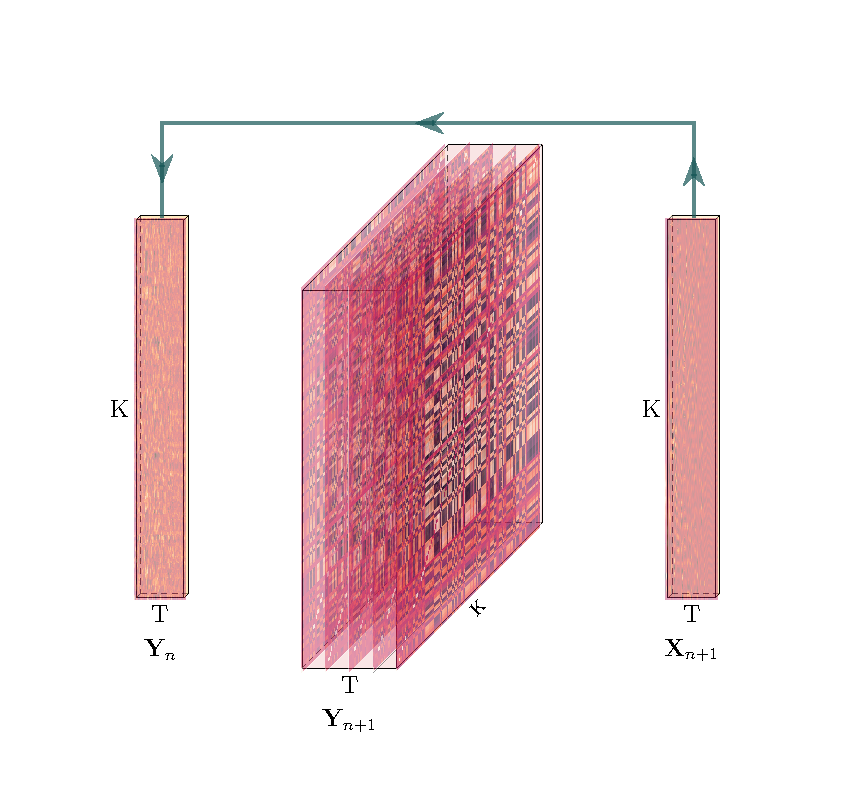
\includegraphics[width=0.4\textwidth]{figs/methods_fig}
  \caption{\textbf{Estimating dynamic high-order correlations.}  Given
    a $T$ by $K$ matrix of multivariate timeseries data,
    $\mathbf{X}_n$ (where $n \in \mathbb{N}, n \geq 0$), we use
    Equation~\ref{eqn:timecorr} to compute a timeseries of
    $K$ by $K$ correlation matrices, $\mathbf{Y}_{n+1}$.  We then
    approximate $\mathbf{Y}_{n+1}$ with the $T$ by $K$ matrix
    $\mathbf{X}_{n+1}$.  This process may be repeated to scalably estimate
    iteratively higher-order correlations in the data.  Note that the
    transposes of $\mathbf{X}_n$ and $\mathbf{X}_{n+1}$ are displayed
    in the figure for compactness.
  \label{fig:methods}}
\end{figure}


\subsection*{Kernel-based approach for computing dynamic correlations}
Given a $T$ by $K$ matrix of observations, $\mathbf{X}$, we can compute the (static)
Pearson's correlation between any pair of columns, $\mathbf{X}(\cdot, i)$ and
$\mathbf{X}(\cdot, j)$ using~\citep{Pear01}:
\begin{align}
  \mathrm{corr}(\mathbf{X}(\cdot, i), \mathbf{X}(\cdot, j)) &=
                                                              \frac{\sum_{t=1}^T
                                                              \left(\mathbf{X}(t,
                                                              i)
                                                              -
                                                              \bar{\mathbf{X}}(\cdot,
                                                              i)\right)
                                                              \left(\mathbf{X}(t,
                                                              j)
                                                              -
                                                              \bar{\mathbf{X}}(\cdot, j)\right)}{\sqrt{\sum_{t=1}^T
                                                              \sigma^2_{\mathbf{X}(\cdot, i)} 
                                                              \sigma^2_{\mathbf{X}(\cdot, j)}}},~\mathrm{where}\\\label{eqn:corr}
  \bar{\mathbf{X}}(\cdot, k) &= \frac{1}{T}\sum_{t=1}^T
                               \mathbf{X}(t, k),~\mathrm{and}\\
  \sigma^2_{\mathbf{X}(\cdot, k)} &= \frac{1}{T}\sum_{t=1}^T \left( \mathbf{X}(t, k) -
                                    \bar{\mathbf{X}}(\cdot, k) \right)^2 
\end{align}
We can generalize this formula to compute time-varying correlations by
incorporating a \textit{kernel function} that takes a time $t$ as
input, and returns how much the observed data at each timepoint
$\tau \in \left[ -\infty, \infty \right]$ contributes to the estimated instantaneous
correlation at time $t$~\citep[Fig.~\ref{fig:kernels}; also see][for a
similar approach]{AlleEtal12b}.
\begin{figure}
  \centering
  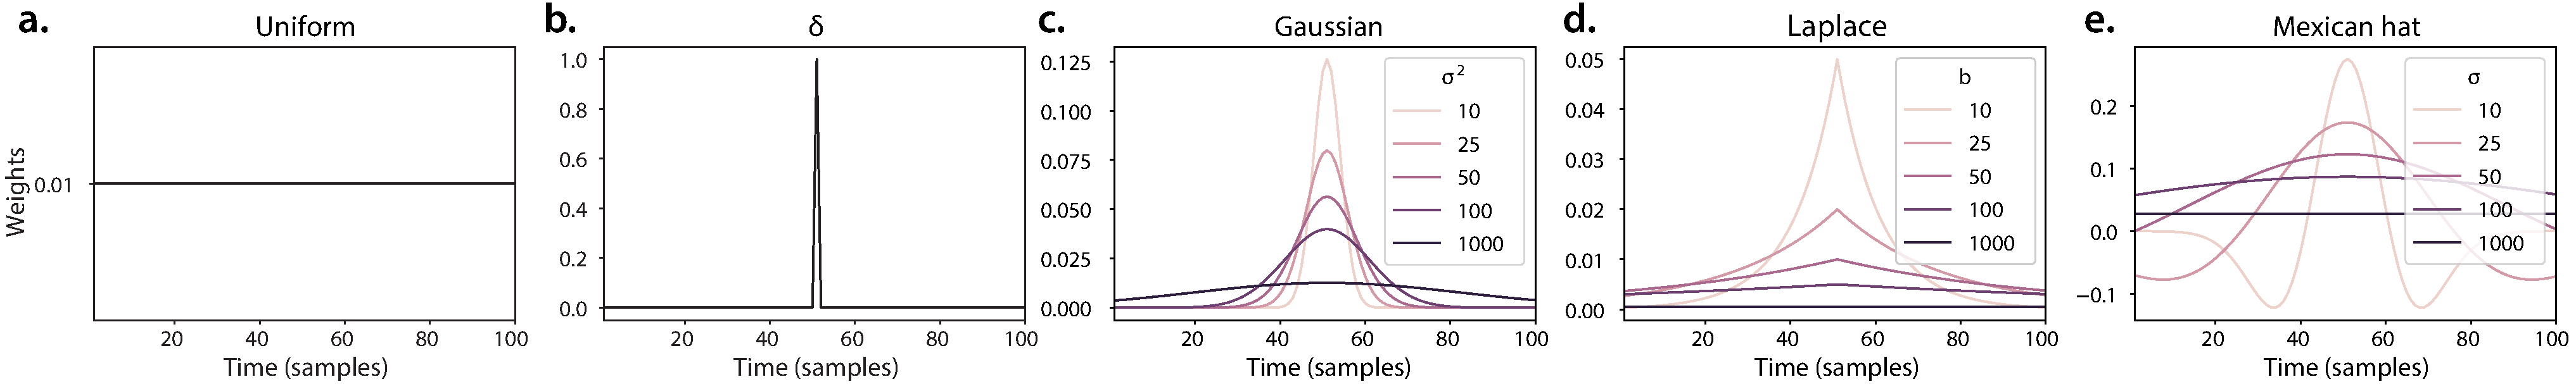
\includegraphics[width=\textwidth]{figs/kernels}
  \caption{\textbf{Examples of kernel functions.} Each panel displays
    per-timepoint weights for a kernel centered at $t = 50$, evaluated
    at 100 timepoints ($\tau \in \left[1, ..., 100\right]$).
    \textbf{a. Uniform kernel.} The weights are timepoint-invariant;
    observations at all timepoints are weighted equally, and do not
    change as a function of $\tau$.  This is a special case kernel
    function that reduces dynamic correlations to static correlations.
    \textbf{b. Dirac $\delta$ kernel.} Only the observation at
    timepoint $t$ is given a non-zero weight (of 1).
    \textbf{c. Gaussian kernels.} Each kernel's weights fall off in
    time according to a Gaussian probability density function centered
    on time $t$.  Weights derived using several different example
    width parameters ($\sigma^2$) are displayed.  \textbf{d. Laplace
      kernels.}  Each kernel's weights fall off in time according to a
    Laplace probability density function centered on time $t$.
    Weights derived using several different example width parameters
    ($b$) are displayed.  \textbf{e. Mexican hat (Ricker wavelet)
      kernels.}  Each kernel's weights fall off in time according to a
    Ricker wavelet centered on time $t$.  This function highlights the
    \textit{contrasts} between local versus surrounding activity
    patterns in estimating dynamic correlations. Weights derived using
    several different example width parameters ($\sigma$) are
    displayed.}
  \label{fig:kernels}
\end{figure}

Given a kernel function $\kappa_t(\cdot)$ for timepoint $t$,
evaluated at timepoints $\tau \in \left[ 1, ..., T \right]$, we
can update the static correlation formula in Equation~\ref{eqn:corr}
to estimate the \textit{instantaneous correlation} at timepoint $t$:
\begin{align}
  \mathrm{timecorr}_{\kappa_t}\left(\mathbf{X}(\cdot, i), \mathbf{X}(\cdot, j)\right) &= \frac{\sum_{\tau=1}^T \left( \mathbf{X}(\tau, i) -
                                       \widetilde{\mathbf{X}}_{\kappa_t}(\cdot,
                                                                                        i) \right)
                                 \left( \mathbf{X}(\tau, j) -
                                        \widetilde{\mathbf{X}}_{\kappa_t}(\cdot,
                                                                                        j)\right)}
              {\sqrt{\sum_{\tau=1}^T
                                              \widetilde{\sigma}_{\kappa_t}^2(\mathbf{X}(\cdot,
                                                                                        i))
                                              \widetilde{\sigma}_{\kappa_t}^2(\mathbf{X}(\cdot, j))}},~\mathrm{where}\label{eqn:timecorr}\\
  \widetilde{\mathbf{X}}_{\kappa_t}(\cdot, k) &= \sum_{\tau=1}^T
                       \kappa_t(\tau)\mathbf{X}(\tau, k),\\
  \widetilde{\sigma}_{\kappa_t}^2(\mathbf{X}(\cdot, k)) &= \sum_{\tau=1}^T
                                                  \left(
                                                  \mathbf{X}(\tau, k) -
                            \widetilde{\mathbf{X}}_{\kappa_t}(\cdot, k) \right)^2.
\end{align}
Here
$\mathrm{timecorr}_{\kappa_t}(\mathbf{X}(\cdot, i), \mathbf{X}(\cdot,
j))$ reflects the correlation at time $t$ between columns $i$ and $j$
of $\mathbf{X}$, estimated using the kernel $\kappa_t$.  We evaluate
Equation~\ref{eqn:timecorr} in turn each pair of columns in
$\mathbf{X}$ and for kernels centered on each timepoint in the
timeseries, respectively, to obtain a $T$ by $K$ by $K$ timeseries of
dynamic correlations, $\mathbf{Y}$.  For convenience, we then reshape
the upper triangles and diagonals of each timepoint's correlation matrix into a row
vector to obtain an equivalent $T$ by $\left( \frac{K^2 - K}{2} + K \right)$ matrix.

\subsubsection*{Dynamic inter-subject functional connectivity (DISFC)}
Equation~\ref{eqn:timecorr} provides a means of taking a single
observation matrix, $\mathbf{X}_n$ and estimating the dynamic
correlations from moment to moment, $\mathbf{Y}_{n+1}$.  Suppose that
one has access to a set of multiple observation matrices that reflect
the same phenomenon.  For example, one might collect neuroimaging data
from several experimental participants, as each participant performs
the same task (or sequence of tasks).  Let $\mathbf{X}_n^1$,
$\mathbf{X}_n^2$, ..., $\mathbf{X}_n^P$ reflect the $T$ by $K$
observation matrices ($n = 0$) or reduced correlation matrices
($n > 0$) for each of $P$ participants in an experiment.  We can use
\textit{inter-subject functional connectivity}~\citep[ISFC;
][]{SimoEtal16} to compute the stimulus-driven correlations reflected
in the multi-participant dataset at a given timepoint $t$ using:
\begin{align}
\bar{\mathbf{C}}(t) = M\left(R\left(\frac{1}{2P} \sum_{p=1}^P
  Z\left(\mathbf{Y}_{n+1}^p(t)\right)^\mathrm{T} + Z\left(\mathbf{Y}_{n+1}^p(t)\right)\right)\right),\label{eqn:disfc}
\end{align}
where $M$ extracts and vectorizes the upper triangle and diagonal of a symmetric
matrix, $Z$ is the Fisher $z$-transformation~\citep{Zar10}:
\begin{align}
Z(r) = \frac{\log(1+r) - \log(1-r)}{2}
\end{align}
$R$ is the inverse of $Z$:
\begin{align}
R(z) = \frac{\exp(2z - 1)}{\exp(2z + 1)},
\end{align}
and $\mathbf{Y}_{n+1}^p(t)$ denotes the correlation matrix at timepoint $t$
(Eqn.~\ref{eqn:timecorr}) between each column of $\mathbf{X}_n^p$ and each
column of the average $\mathbf{X}_n$ from all \textit{other}
participants, $\bar{\mathbf{X}}_n^{ \backslash p}$:
\begin{align}
  \bar{\mathbf{X}}_n^{ \backslash p} = R\left(\frac{1}{P-1}\sum_{q \in
  \backslash p} Z\left( \mathbf{X}_n^q \right) \right),
\end{align}
where $\backslash p$ denotes the set of all participants other than
participant $p$. In this way, the $T$ by $\left( \frac{K^2 - K}{2} + K \right)$ DISFC
matrix $\bar{\mathbf{C}}$ provides a time-varying extension of the ISFC
approach developed by \cite{SimoEtal16}.

\subsection*{Low-dimensional representations of dynamic
  correlations}

Given a $T$ by $\left( \frac{K^2 - K}{2} + K \right)$ matrix of
dynamic correlations, $\mathbf{Y}_n$, we propose two general
approaches to computing a $T$ by $K$ low-dimensional representation of
those correlations, $\mathbf{X}_n$.  The first approach uses
dimensionality reduction algorithms to project $\mathbf{Y}_n$ onto a
$K$-dimensional space.  The second approach uses graph measures to
characterize the relative positions of each feature
($k \in \left[1, ..., K \right]$) in the network defined by the
correlation matrix at each timepoint.

\subsubsection*{Dimensionality reduction-based approaches to computing
  $\mathbf{X}_n$}

The modern toolkit of dimensionality reduction algorithms include
Principal Components Analysis~\citep[PCA;][]{Pear01}, Probabilistic
PCA~\citep[PPCA;][]{TippBish99}, Exploratory Factor
Analysis~\citep[EFA;][]{Spea04}, Independent Components
Analysis~\citep[ICA;][]{JuttHera91, ComoEtal91}, $t$-Stochastic
Neighbor Embedding~\citep[$t$-SNE;][]{MaatHint08}, Uniform Manifold
Approximation and Projection~\citep[UMAP;][]{McInHeal18}, non-negative
matrix factorization~\citep[NMF;][]{LeeSeun99}, Topographic Factor
Analysis~\cite[TFA;][]{MannEtal14b}, Hierarchical Topographic Factor
analysis~\cite[HTFA;][]{MannEtal18}, Topographic Latent Source
Analysis~\cite[TLSA;][]{GersEtal11}, dictionary
learning~\citep{MairEtal09a, MairEtal09b}, and deep
auto-encoders~\citep{HintSala06}, among others.  While complete
characterizations of each of these algorithms is beyond the scope of
the present manuscript, the general intuition driving these approaches
is to compute the $T$ by $K$ matrix, $\mathbf{X}$, that is closest to
the original $T$ by $J$ matrix, $\mathbf{Y}$, where (typically)
$K \ll J$.  The different approaches place different constraints on
what properties $\mathbf{X}$ must satisfy and which aspects of the
data are compared (and how) in order to optimize how well
$\mathbf{X}$ approximates $\mathbf{Y}$.

Applying dimensionality reduction algorithms to $\mathbf{Y}$ yields an
$\mathbf{X}$ whose columns reflect weighted combinations (or nonlinear
transformations) of the original columns of $\mathbf{Y}$.  This has
two main consequences.  First, with each repeated dimensionality
reduction, the resulting $\mathbf{X}_n$ has lower and lower fidelity
(with respect to what the ``true'' $\mathbf{Y}_n$ might have looked
like without using dimensionality reduction to maintain scalability).
In other words, computing $\mathbf{X}_n$ is a lossy operation.
Second, whereas each columns of $\mathbf{Y}_n$ may be mapped
directly onto specific pairs of columns of $\mathbf{X}_{n-1}$, the
columns of $\mathbf{X}_n$ reflect weighted combinations and/or
nonlinear transformations of the columns of $\mathbf{Y}_n$.  Many
dimensionality reduction algorithms are invertible (or approximately
invertible).  However, attempting to map a given $\mathbf{X}_n$ back
onto the original feature space of $\mathbf{X}_0$ will usually require
$\mathcal{O}(TK^{2n})$ space and therefore quickly becomes intractable
as $n$ or $K$ grow large.

\subsubsection*{Graph measure approaches to computing
  $\mathbf{X}_n$}
The above dimensionality reduction approaches to approximating a given
$\mathbf{Y}_n$ with a lower-dimensional $\mathbf{X}_n$ preserve a
(potentially recombined and transformed) mapping back to the original
data in $\mathbf{X}_0$.  We also explore graph measures that instead
characterize each feature's relative \textit{position} in the broader
network of interactions and connections.  To illustrate the
distinction between the two general approaches we explore, suppose a
network comprises nodes $A$, $B$, and $C$.  If $A$ and $B$ exhibit
uncorrelated activity patterns, the functional connection
(correlation) between them will be (by definition) close to 0.
However, if $A$ and $B$ each interact with $C$ in similar ways, we
might attempt to capture those similarities using a measure that
reflects how $A$ and $B$ interact with \textit{other} members of the
network.

In general, graph measures take as input a matrix of
interactions (e.g., using the above notation, a $K$ by $K$
correlation matrix or binarized correlation matrix reconstituted from
a single timepoint's row of $\mathbf{Y}$) and return as output a set
of $K$ measures describing how each node (feature) sits within that
correlation matrix with respect to the rest of the population.  Widely
used measures include betweenness centrality~\citep[the proportion of
shortest paths between each pair of nodes in the population that
involves the given node in question; e.g.,][]{Newm05, OpsaEtal10,
  Bart04, GeisEtal08, Free77}; diversity and
dissimilarity~\citep[characterizations of how differently connected a
given node is from others in the population; e.g.,][]{Rao82, Lin09,
  RicoSzei06}; Eigenvector centrality and pagerank
centrality~\citep[measures of how influential a given node is within
the broader network; e.g.,][]{Newm08, Bona07, LohmEtal10,
  HaluEtal13}; transfer entropy and flow coefficients~\citep[a measure
of how much information is flowing from a given node to other nodes in
the network; e.g.,][]{HoneEtal07, Schr00}; $k$-coreness
centrality~\citep[a measure of the connectivity of a node within its
local sub-graph; e.g.,][]{AlvaEtal05, ChriFowl10}; within-module
degree~\citep[a measure of how many connections a node has to its
close neighbors in the network; e.g.,][]{RubiSpor10}; participation
coefficient~\citep[a measure of the diversity of a node's connections
to different sub-graphs in the network; e.g.,][]{RubiSpor10}; and
sub-graph centrality~\citep[a measure of a node's participation in all
of the network's sub-graphs; e.g.,][]{EstrRodr05}; among others.

For a given graph measure,
$\eta: \mathbb{R}^{K \times K} \rightarrow \mathbb{R}^K$, we can use
$\eta$ to tranform each row of $\mathbf{Y}_n$ in a way that
characterizes the corresponding graph properties of each
column.  This results in a new $T$ by $K$ matrix, $\mathbf{X}_n$, that
reflects how the features reflected in the columns of $\mathbf{X}_{n-1}$
participate in the network during each timepoint (row).


\subsection*{Dynamic higher-order correlations}

Because $\mathbf{X}_n$ has the same shape as the original data
$\mathbf{X}_0$, approximating $\mathbf{Y}_n$ with a lower-dimensional
$\mathbf{X}_n$ enables us to estimate high-order dynamic correlations
in a scalable way.  Given a $T$ by $K$ input matrix, the output of
Equation~\ref{eqn:timecorr} requires $\mathcal{O}(TK^2)$ space to
store.  Repeated applications of Equation~\ref{eqn:timecorr} (i.e.,
computing dynamic correlations between the columns of the outputted
dynamic correlation matrix) each require exponentially more space; in
general the $n^\mathrm{th}$-order dynamic correlations of a $T$ by $K$
timeseries occupies $\mathcal{O}(TK^{2n})$ space.  However, when we
approximate or summarize the output of Equation~\ref{eqn:timecorr} with a $T$ by
$K$ matrix (as described above), it becomes feasible to compute even
very high-order correlations in high-dimensional data.  Specifically,
approximating the $n^\mathrm{th}$-order dynamic correlations of a $T$
by $K$ timeseries requires only $\mathcal{O}(TK^2)$ additional space--
the same as would be required to compute first-order dynamic
correlations. In other words, the space required to store $n+1$
multivariate timeseries reflecting up to $n^\mathrm{th}$ order
correlations in the original data scales linearly with $n$ using our
approach (Fig.~\ref{fig:methods}).

\subsection*{Data}
We examined two types of data: synthetic data and human functional
neuroimaging data.  We constructed and leveraged the synthetic data to
evaluate our general approach~\citep[for a related validation
approach see][]{ThomEtal18}.  Specifically, we tested how well
Equation~\ref{eqn:timecorr} could be used to recover known dynamic
correlations using different choices of kernel ($\kappa$;
Fig.~\ref{fig:kernels}), for each of several synthetic datasets that
exhibited different temporal properties.  We applied our approach to a
functional neuroimaging dataset to test the hypothesis that ongoing
cognitive processing is reflected in high-order dynamic correlations.
We used an across-participant classification test to estimate whether
dynamic correlations of different orders contain information about
which timepoint in a story participants were listening to.

\subsubsection*{Synthetic data}
We constructed a total of 40 different multivariate timeseries,
collectively reflecting a total of 4 qualitatively different patterns
of dynamic correlations (i.e., 10 datasets reflecting each type of
dynamic pattern).  Each timeseries comprised 50 features (dimensions)
that varied over 300 timepoints.  The observations at each timepoint
were drawn from a zero-mean multivariate Gaussian distribution with a
covariance matrix defined for each timepoint as described below.  We
drew the observations at each timepoint independently from the draws
at all other timepoints; in other words, for each observation
$s_t \sim \mathcal{N}\left(\mathbf{0}, \mathbf{\Sigma}_t\right)$ at
timepoint $t$, $p(s_t) = p(s_t | s_{\backslash t})$.

\paragraph*{Constant.}  We generated data with stable underlying
correlations to evaluate how Equation~\ref{eqn:timecorr} characterized
correlation ``dynamics'' when the ground truth correlations were
static.  We constructed 10 multivariate timeseries whose observations
were each drawn from a single (stable) Gaussian distribution.  For
each dataset (indexed by $m$), we constructed a random covariance matrix,
$\mathbf{\Sigma}_m$:
\begin{align}
  \mathbf{C}(i, j) &\sim \mathcal{N}(0, 1)\\
  \mathbf{\Sigma}_m &= \mathbf{C}
                                          \mathbf{C}^\top~\mathrm{, where}\label{eqn:randcorr}
  \end{align}
  $i, j \in \left[1, 2, ..., 50 \right]$.  In other words, all of the
  observations (for each of the 300 timepoints) within each dataset
  were drawn from a multivariate Gaussian distribution with the same
  covariance matrix, and the 10 datasets each used a different
  covariance matrix.
  
  \paragraph*{Random.}  We generated a second set of 10 synthetic
  datasets whose observations at each timepoint were drawn from a
  Gaussian distribution with a new randomly constructed (using
  Eqn.~\ref{eqn:randcorr}) covariance matrix.  Because each
  timepoint's covariance matrix was drawn independently from the
  covariance matrices for all other timepoints, these datasets
  provided a test of reconstruction accuracy in the absence of any
  meaningful underlying temporal structure in the dynamic correlations
  underlying the data.
  
  \paragraph*{Ramping.}  We generated a third set of 10 synthetic
  datasets whose underlying correlations changed gradually over time.
  For each dataset, we constructed two \textit{anchor} correlation
  matrices using Equation~\ref{eqn:randcorr},
  $\mathbf{\Sigma}_{\mathrm{start}}$ and
  $\mathbf{\Sigma}_{\mathrm{end}}$.  For each of the 300 timepoints in
  each dataset, we drew the observations from a multivariate Gaussian
  distribution whose covariance matrix at each timepoint $t \in
  \left[0, ..., 299\right]$ was given by
  \begin{align}
    \mathbf{\Sigma}_t = \left( 1 - \frac{t}{299} \right)
    \mathbf{\Sigma}_{\mathrm{start}} + \frac{t}{299}\mathbf{\Sigma}_{\mathrm{end}}.
  \end{align}
The gradually changing correlations underlying these datasets allow us
to evaluate the recovery of dynamic correlations when each timepoint's
correlation matrix is unique (as in the random datasets), but where
the correlation dynamics are structured.
  
\paragraph*{Event.} We generated a fourth set of 10 synthetic datasets
whose underlying correlation matrices exhibited prolonged intervals of
stability, interspersed with abrupt changes.  For each dataset, we
used Equation~\ref{eqn:randcorr} to generate 5 random covariance
matrices.  We constructed a timeseries where each set of 60 consecutive samples
was drawn from a Gaussian with the same covariance matrix.  These
datasets were intended to simulate a system that undergoes occasional
abrupt state changes.

\subsubsection*{Functional neuroimaging data collected during story
  listening}
We examined an fMRI dataset collected by \cite{SimoEtal16} that the
authors have made publicly available at
\href{http://arks.princeton.edu/ark:/88435/dsp015d86p269k}{arks.princeton.edu/ark:/88435/dsp015d86p269k}.  The dataset
comprises neuroimaging data collected as participants listened
to an audio recording of a story (intact condition; 36 participants),
listened to time scrambled recordings of the same story (17
participants in the paragraph-scrambled condition listened to the
paragraphs in a randomized order and 36 in the word-scrambled
condition listened to the words in a randomized order), or lay resting
with their eyes open in the scanner (rest condition; 36
participants).  Full neuroimaging details may be found in the original
paper for which the data were collected~\citep{SimoEtal16}.

\paragraph{Hierarchical topographic factor analysis (HTFA).}
Following our prior related work, we used HTFA~\citep{MannEtal18} to
derive a compact representation of the neuroimaging data.  In brief,
this approach approximates the timeseries of voxel activations (44,415
voxels) using a much smaller number of radial basis function (RBF)
nodes~\citep[in this case, 700 nodes, as determined by an optimization
procedure described by][]{MannEtal18}.  This provides a convenient
representation for examining full-brain network dynamics.  All of the
analyses we carried out on the neuroimaging dataset were performed in
this lower-dimensional space.  In other words, each participant's data
matrix, $\mathbf{X}_0$, was a number-of-timepoints by 700 matrix of
HTFA-derived factor weights (where the row and column labels were
matched across participants).  Code for carrying out HTFA on fMRI data
may be found as part of the BrainIAK toolbox~\citep{brainiak}, which
may be downloaded at \href{https://brainiak.org/}{brainiak.org}.

\subsection*{Temporal decoding}
We sought to identify neural patterns that reflected participants'
ongoing cognitive processing of incoming stimulus information.  As
reviewed by \cite{SimoEtal16}, one way of homing in on these
stimulus-driven neural patterns is to compare activity patterns across
individuals (e.g., using ISFC analyses).  In particular, neural
patterns will be similar across individuals to the extent that the
neural patterns under consideration are stimulus-driven, and to the
extent that the corresponding cognitive representations are reflected
in similar spatial patterns across people.  Following this logic, we
used an across-participant temporal decoding test developed by
\cite{MannEtal18} to assess the degree to which different neural
patterns reflected ongoing stimulus-driven cognitive processing across
people.  The approach entails using a subset of the data to train a
classifier to decode stimulus timepoints (i.e., moment in the story
participants listened to) from neural patterns.  We use decoding
(forward inference) accuracy on held-out data, from held-out
participants, as a proxy for the extent to which the inputted neural
patterns reflected stimulus-driven cognitive processing in a similar
way across individuals.

\subsubsection*{Forward inference and decoding accuracy}
We used an across-participant correlation-based classifier to decode
which stimulus timepoint matched each timepoint's neural pattern.  We
first divided the participants into two groups: a template group,
$\mathcal{G}_{\mathrm{template}}$, and a to-be-decoded group,
$\mathcal{G}_{\mathrm{decode}}$.  We used Equation~\ref{eqn:disfc} to
compute a DISFC matrix for each group
($\bar{\textbf{C}}_{\mathrm{template}}$ and
$\bar{\textbf{C}}_{\mathrm{decode}}$, respectively).  We then
correlated the rows of $\bar{\textbf{C}}_{\mathrm{template}}$ and
$\bar{\textbf{C}}_{\mathrm{decode}}$ to form a number-of-timepoints by
number-of-timepoints decoding matrix, $\mathbf{\Lambda}$.  In this
way, the rows of $\mathbf{\Lambda}$ reflected timepoints from the
template group, while the columns reflected timepoints from the
to-be-decoded group.  We used $\mathbf{\Lambda}$ to assign temporal
labels to each row $\bar{\textbf{C}}_{\mathrm{decode}}$ using the row
of $\bar{\textbf{C}}_{\mathrm{template}}$ with which it was most
highly correlated.  We then repeated this decoding procedure, but
using $\mathcal{G}_{\mathrm{decode}}$ as the template group and
$\mathcal{G}_{\mathrm{template}}$ as the to-be-decoded group.  Given
the true timepoint labels (for each group), we defined the
\textit{decoding accuracy} as the average proportion of correctly
decoded timepoints, across both groups.  We defined the
\textit{relative decoding accuracy} as the difference between the
decoding accuracy and chance accuracy (i.e., $\frac{1}{T}$).

\subsubsection*{Feature weighting and testing}
We sought to examine which types of neural features (i.e.,
activations, first-order dynamic correlations, and higher-order
dynamic correlations) were informative to the temporal decoders.
Using the notation above, these features correspond to $\mathbf{X}_0$,
$\mathbf{X}_1$, $\mathbf{X}_2$, $\mathbf{X}_3$, and so on.

One challenge to fairly evaluating high-order correlations is that if
the kernel used in Equation~\ref{eqn:timecorr} is wider than a single
timepoint, each repeated application of the equation will result in
further temporal blur.  Because our primary assessment metric is
temporal decoding accuracy, this unfairly biases against detecting
meaningful signal in higher-order correlations (relative to
lower-order correlations).  We attempted to mitigate temporal blur in
estimating each $\mathbf{X}_n$ by using a Dirac $\delta$ function
kernel (which places all of its mass over a single timepoint;
Fig.~\ref{fig:kernels}b) to compute each lower-order correlation
($\mathbf{X}_1, \mathbf{X}_2, ..., \mathbf{X}_{n-1}$).  We then used a
new (potentially wider, as described below) kernel to compute
$\mathbf{X}_{n}$ from $\mathbf{X}_{n-1}$.  In this way, temporal
blurring was applied only in the last step of computing
$\mathbf{X}_n$.  We note that, because each $\mathbf{X}_n$ is a
low-dimensional representation of the corresponding $\mathbf{Y}_n$,
the higher-order correlations we estimated reflect true correlations
in the data with lower-fidelity than estimates of lower-order
correlations.  Therefore, even after correcting for temporal blurring,
our approach is still biased against finding meaningful signal in
higher-order correlations.

After computing each
$\mathbf{X}_1, \mathbf{X}_2, ..., \mathbf{X}_{n-1}$ for each
participant, we divided participants into two equally sized groups
($\pm 1$ for odd numbers of participants):
$\mathcal{G}_{\mathrm{train}}$ and $\mathcal{G}_{\mathrm{test}}$.  We
then further subdivided $\mathcal{G}_{\mathrm{train}}$ into
$\mathcal{G}_{\mathrm{train}_1}$ and $\mathcal{G}_{\mathrm{train}_2}$.
We then computed $\mathbf{\Lambda}$ (temporal correlation) matrices
for each type of neural feature, using
$\mathcal{G}_{\mathrm{train}_1}$ and $\mathcal{G}_{\mathrm{train}_2}$.
This resulted in $n+1$ $\mathbf{\Lambda}$ matrices (one for the
original timeseries of neural activations, and one for each of $n$
orders of dynamic correlations).  Our objective was to find a set of
weights for each of these $\mathbf{\Lambda}$ matrices such that the
weighted average of the $n+1$ matrices yielded the highest decoding
accuracy.  We used quasi-Newton gradient ascent~\citep{NoceWrig06},
using decoding accuracy (for $\mathcal{G}_{\mathrm{train}_1}$ and
$\mathcal{G}_{\mathrm{train}_2}$) as the objective function to be
maximized, to find an optimal set of training data-derived weights,
$\phi_{0, 1, ..., n}$, where $\sum_{i=0}^n \phi_i = 1$ and where
$\phi_i \geq 0 \forall i \in \left[0, 1, ..., n\right]$.

After estimating an optimal set of weights, we computed a new set of
$n + 1$ $\mathbf{\Lambda}$ matrices correlating the DISFC patterns
from $\mathcal{G}_{\mathrm{train}}$ and $\mathcal{G}_{\mathrm{test}}$
at each timepoint.  We use the resulting decoding accuracy of
$\mathcal{G}_{\mathrm{test}}$ timepoints to estimate how informative
the set of neural features containing up to $n^\mathrm{th}$ order
correlations were.

We used a permutation-based procedure to form stable estimates of
decoding accuracy for each set of neural features.  In particular, we
computed the decoding accuracy for each of 10 random group assignments of
$\mathcal{G}_{\mathrm{train}}$ and $\mathcal{G}_{\mathrm{test}}$.  We
report the mean accuracy (along with 95\% confidence intervals) for each set
of neural features.


\subsubsection*{Identifying robust decoding results}
The temporal decoding procedure we use to estimate which neural
features support ongoing cognitive processing is governed by several
parameters. In particular, Equation~\ref{eqn:timecorr} requires
defining a kernel function, which can take on different shapes and
widths.  For a fixed set of neural features, each of these parameters
can yield different decoding accuracies.  Further, the best decoding
accuracy for a given timepoint may be reliably achieved by one set of
parameters, whereas the best decoding accuracy for another timepoint
might be reliably achieved by a different set of parameters, and the
best decoding accuracy across \textit{all} timepoints might be
reliably achieved by still another different set of parameters.
Rather than attempting to maximize decoding accuracy, we sought to
discover the trends in the data that were robust to classifier
parameters choices.  Specifically, we sought to characterize how
decoding accuracy varied (under different experimental conditions) as
a function of which neural features were considered.

To identify decoding results that were robust to specific classifier
parameter choices, we repeated our decoding analyses after
substituting in each of a variety of kernel shapes and widths for
Equation~\ref{eqn:timecorr}.  We examined Gaussian
(Fig.~\ref{fig:kernels}c), Laplace (Fig.~\ref{fig:kernels}d), and
Mexican Hat (Fig.~\ref{fig:kernels}e) kernels, each with widths of 5,
10, 20, and 50 samples.  We then report the average decoding
accuracies across all of these parameter choices.  This enabled us to
(partially) factor out performance characteristics that were
parameter-dependent, within the set of parameters we examined.


\subsubsection*{Reverse inference}
The dynamic patterns we examined comprise high-dimensional correlation
patterns at each timepoint.  To help interpret the resulting patterns
in the context of other studies, we created summary maps by computing
the across-timepoint average pairwise correlations at each order of
analysis (first order, second order, etc.).  We selected the 10
strongest (absolute value) correlations at each order.  Each
correlation is between the dynamic activity patterns (or patterns of
dynamic high-order correlations) measured at two RBF nodes (see
\textit{Hierarchical Topographic Factor Analysis}).  Therefore, the 10
strongest correlations involved up to 20 RBF nodes.  Each RBF defines
a spatial function whose activations range from 0 to 1.  We
thresholded each RBF at 0.999 to construct a map of spherical
components that denoted the endpoints of the 10 strongest
correlations.  We then carried out a meta analysis using
Neurosynth~\citep{RubiEtal17} to identify the 10 terms most commonly
associated with the given map.  This resulted in a set of 10 terms
associated with the average dynamic correlation patterns at each
order.



\section*{Results}
We sought to understand whether high-level cognition is supported by
dynamic patterns of high-order correlations.  To that end, we
developed a computational framework for estimating the dynamics of
stimulus-driven high-order correlations in multivariate timeseries
data (see \textit{Dynamic inter-subject functional connectivity
  (DISFC)} and \textit{Dynamic higher-order correlations}).  We
evaluated the efficacy of this framework at recovering known patterns
in several synthetic datasets (see \textit{Synthetic data}).  We then
applied the framework to a public fMRI dataset collected as
participants listened to an auditorally presented story, listened to a
temporally scrambled version of the story, or underwent a resting
state scan (see \textit{Functional neuroimaging data collected during
  story listening}).  We used the relative decoding accuracies of
classifiers trained on different sets of neural features to estimate
which types of features reflected ongoing cognitive processing.

\subsection*{Recovering known dynamic correlations from synthetic data}
We generated synthetic datasets that differed in how the underlying
correlations changed over time.  For each dataset, we applied
Equation~\ref{eqn:timecorr} with a variety of kernel shapes and
widths.  We assessed how well the true underlying correlations at each
timepoint matched the recovered correlations
(Fig.~\ref{fig:synthetic}).  For every kernel and dataset we tested,
our approach recovered the correlation dynamics we embedded into the
data.  However, the quality of these recoveries varied across
different synthetic datasets in a kernel-dependent way.


\begin{figure}[tp]
  \centering
  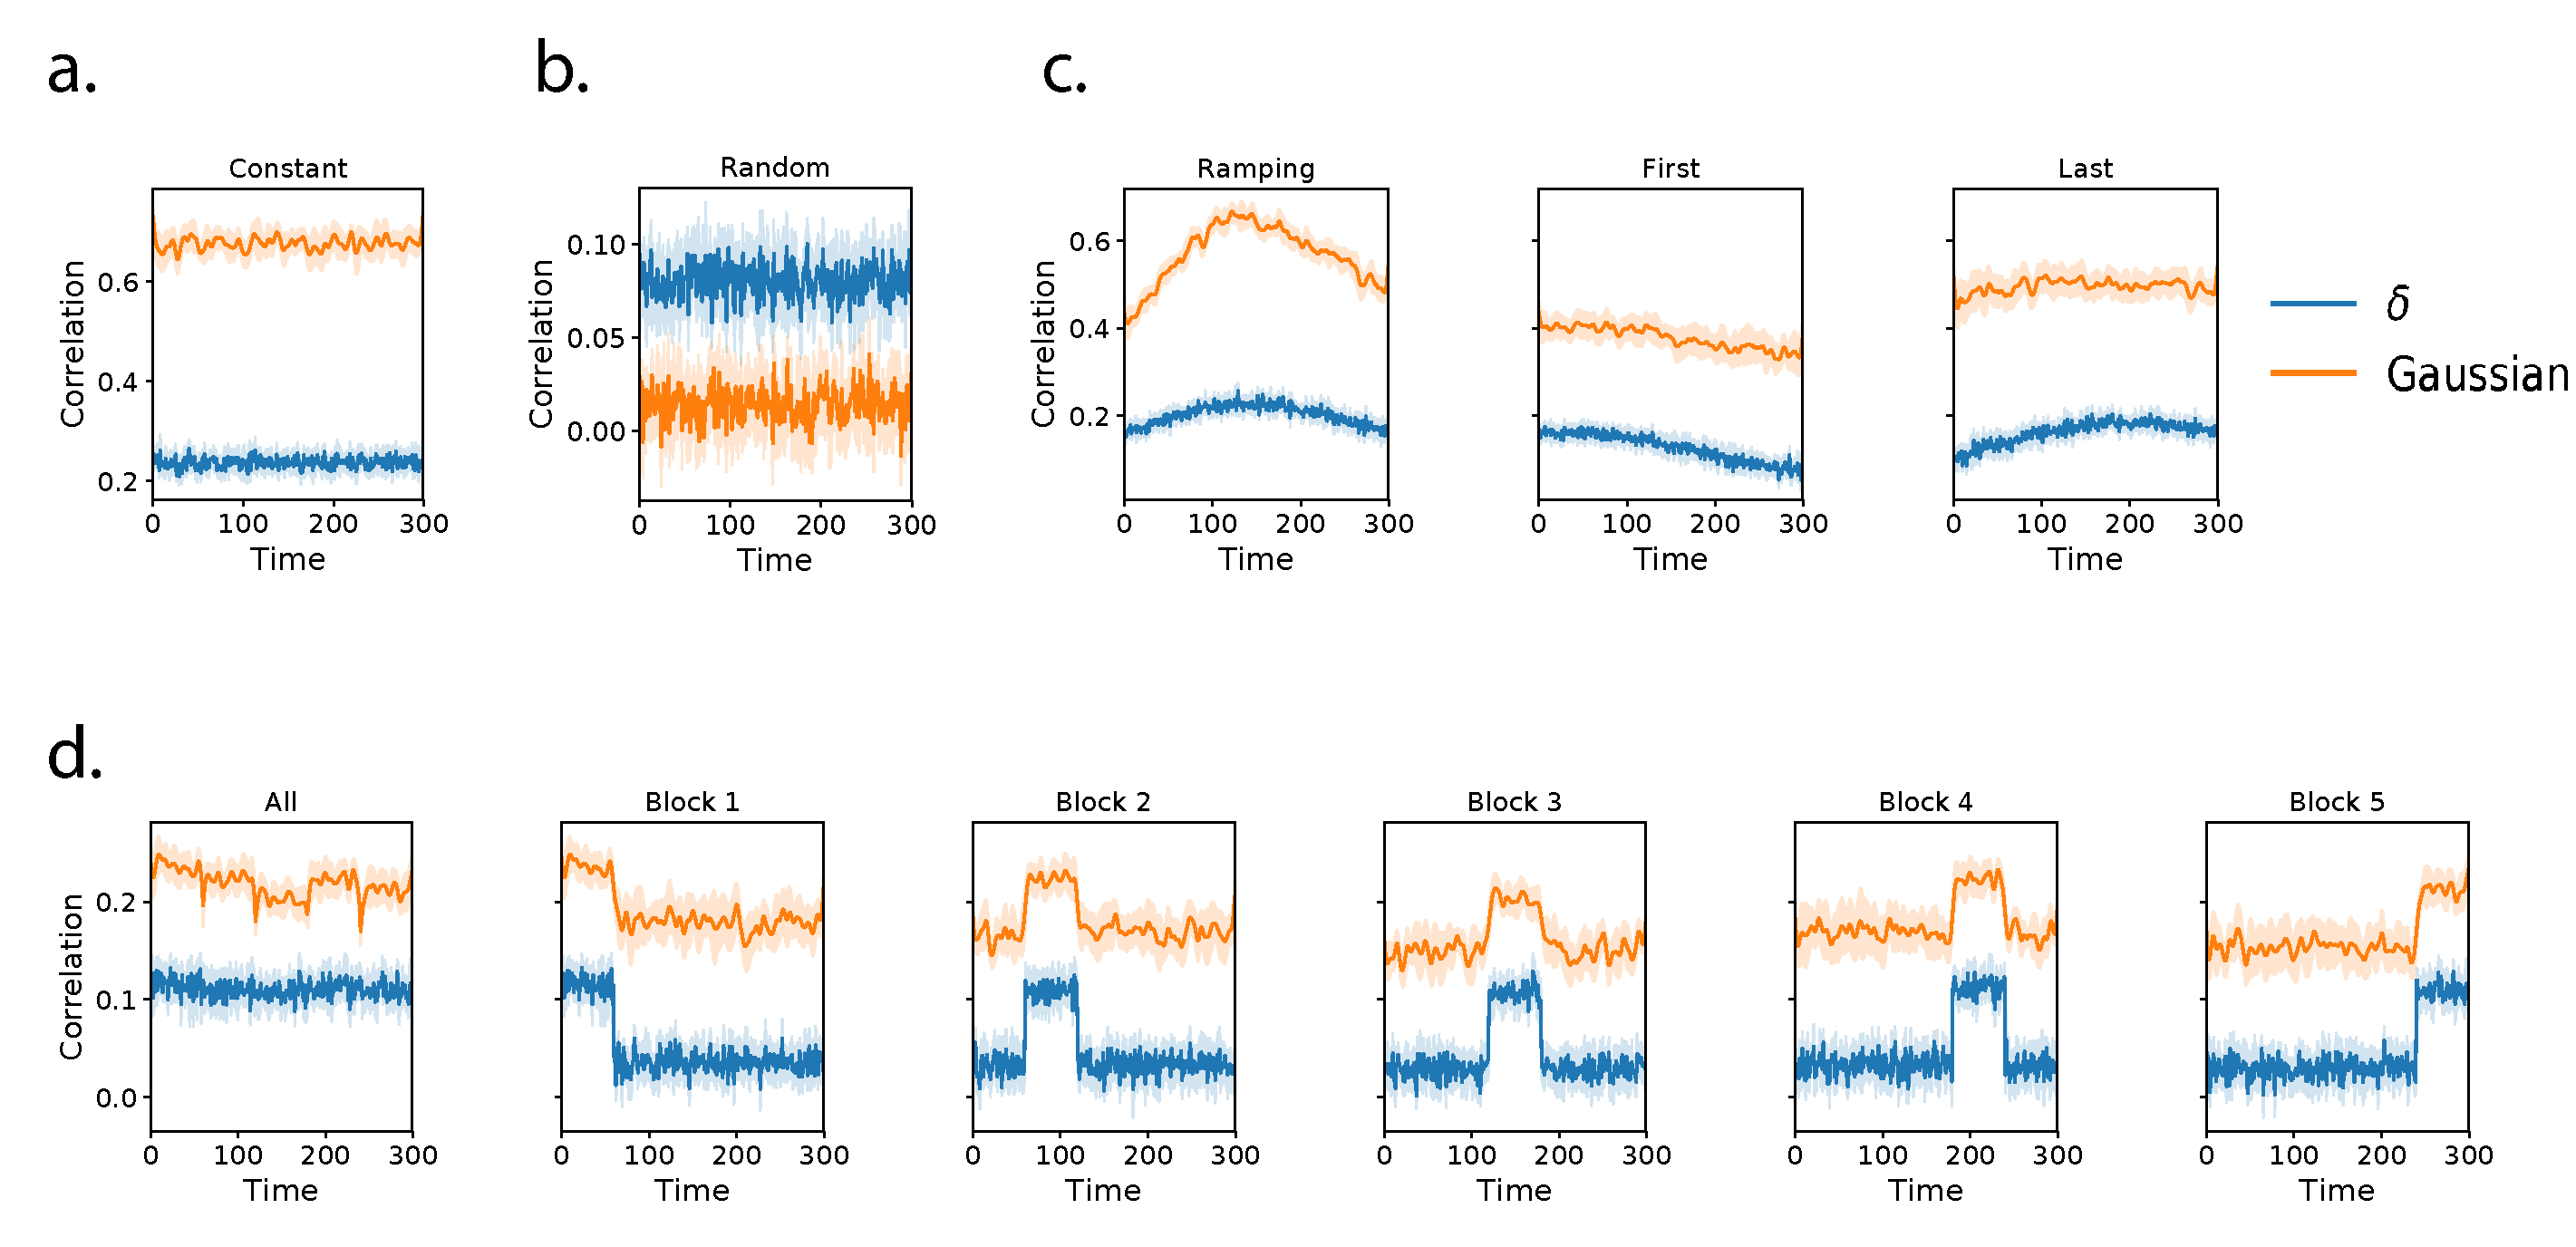
\includegraphics[width=\textwidth]{figs/synthetic_data}
  \caption{\textbf{Recovering known dynamic correlations from
      synthetic data.}  Each panel displays the average correlations
    between the vectorized upper triangles of the recovered
    correlation matrix at each timepoint and either the true
    underlying correlation at each timepoint or a reference
    correlation matrix.  (The averages are taken across 10 different
    randomly generated synthetic datasets of the given category.)
    Error ribbons denote 95\% confidence intervals (taken across
    datasets). Different colors denote different kernel shapes, and
    the shading within each color family denotes the kernel width
    parameter.  For a complete description of each synthetic dataset,
    see \textit{Synthetic data}.  \textbf{a. Constant correlations.}
    These datasets have a stable (unchanging) underlying correlation
    matrix.  \textbf{b. Random correlations.}  These datasets are
    generated using a new independently drawn correlation matrix at
    each new timepoint.  \textbf{c. Ramping correlations.}  These
    datasets are generated by smoothly varying the underlying
    correlations between the randomly drawn correlation matrices at
    first and last timepoints.  The left panel displays the
    correlations between the recovered dynamic correlations and the
    underlying ground truth correlations.  The middle panel compares
    the recovered correlations with the \textit{first} timepoint's
    correlation matrix.  The right panel compares the recovered
    correlations with the \textit{last} timepoint's correlation
    matrix.  \textbf{d. Event-based correlations.}  These datasets are
    each generated using five randomly drawn correlation matrices that
    each remain stable for a fifth of the total timecourse.  The left
    panel displays the correlations between the recovered dynamic
    correlations and the underlying ground truth correlations.  The
    right panels compare the recovered correlations with the
    correlation matrices unique to each event.}
  \label{fig:synthetic}
\end{figure}

In general, wide monotonic kernel shapes (Laplace, Gaussian), and
wider kernels (within a shape), performed best when the correlations
varied gradually from moment-to-moment (Figs.~\ref{fig:synthetic}a, c,
and d).  In the extreme, as the rate of change in correlations
approaches 0 (Fig.~\ref{fig:synthetic}a), an infinitely wide kernel
would exactly recover the Pearson's correlation (e.g., compare
Eqns.~\ref{eqn:corr} and \ref{eqn:timecorr}).

When the correlation dynamics were unstructured in time
(Fig.~\ref{fig:synthetic}b), a Dirac $\delta$ kernel (infinitely
narrow) performed best.  This is because, when every timepoint's
correlations are independent of the correlations at every other
timepoint, averaging data over time dilutes the available signal.
Following a similar pattern, holding kernel shape fixed, narrower
kernel parameters better recovered randomly varying correlations.

\subsection*{Cognitively relevant dynamic high-order correlations in
  fMRI data}
We used across-participant temporal decoders to identify cognitively
relevant neural patterns in fMRI data (see \textit{Forward inference
  and decoding accuracy}).  The dataset we examined~\citep[collected
by][]{SimoEtal16} comprised four experimental conditions that exposed
participants to stimuli that varied systematically in how cognitively
engaging they were.  The \textit{intact} experimental condition had
participants listen to an audio recording of a 10-minute story.  The
\textit{paragraph}-scrambled experimental condition had participants
listen to a temporally scrambled version of the story, where the
paragraphs occurred out of order (but where the same total set of
paragraphs were presented over the full listening interval).  All
participants in this condition experienced the scrambled paragraphs in
the same order.  The \textit{word}-scrambled experimental condition
had participants listen to a temporally scrambled version of the story
where the words in the story occurred in a random order.  All
participants in the word conditions experienced the scrambled words in
the same order.  Finally, in a \textit{rest} experimental condition,
participants lay in the scanner with no overt stimulus, with their
eyes open (blinking as needed).  This dataset provided a convenient
means of testing our hypothesis that different levels of cognitive
processing and engagement are supported by different orders of brain
activity dynamics.

\begin{figure}[tp]
  \centering
  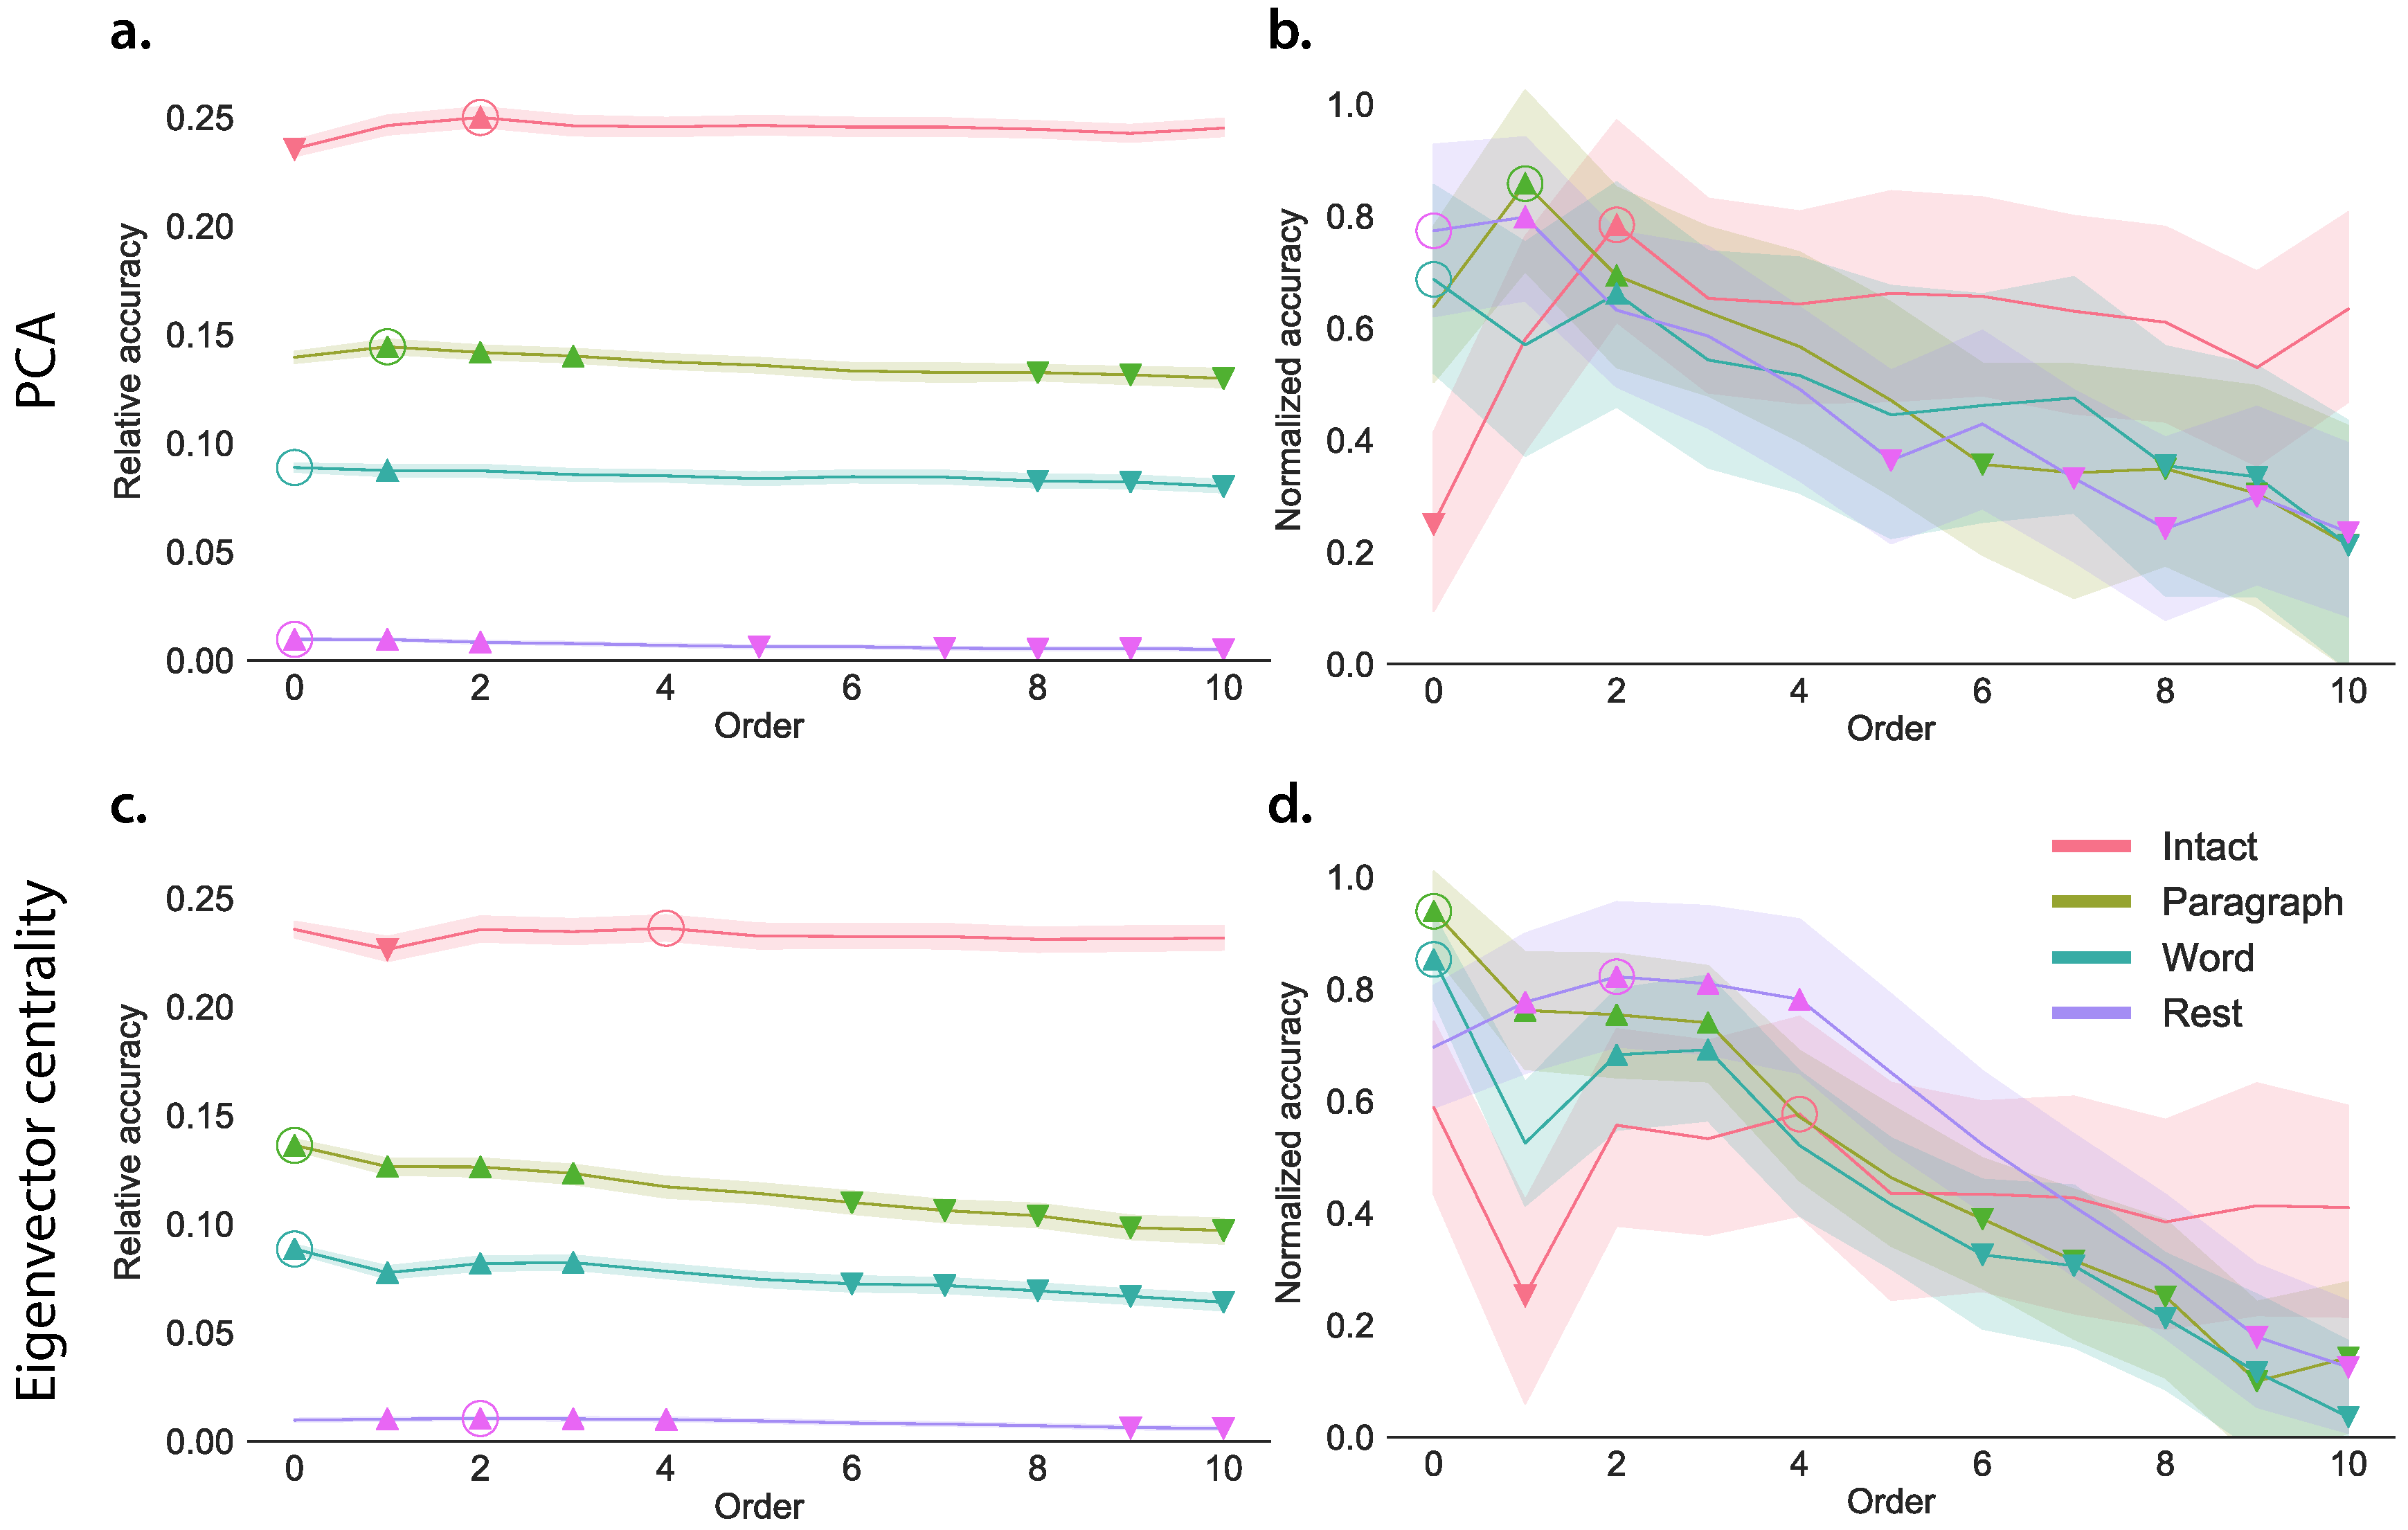
\includegraphics[width=\textwidth]{figs/decode_level}
  \caption{\textbf{Across-participant decoding accuracy varies with
      correlation order and cognitive engagement.}
    \textbf{a.~Decoding accuracy as a function of order: PCA.}
    \textit{Order} ($x$-axis) refers to the maximum order of dynamic
    correlations that were available to the classifiers (see
    \textit{Feature weighting and testing}).  The reported
    across-participant decoding accuracies are averaged over all
    kernel shapes and widths (see \textit{Identifying robust decoding
      results}).  The $y$-values are displayed relative to chance
    accuracy (intact: $\frac{1}{300}$; paragraph: $\frac{1}{272}$;
    word: $\frac{1}{300}$; rest: $\frac{1}{400}$).  The error ribbons
    denote 95\% confidence intervals across cross-validation folds
    (i.e., random assignments of participants to the training and test
    sets).  The colors denote the experimental condition.  Arrows
    denote sets of features that yielded reliably higher (upwards
    facing) or lower (downward facing) decoding accuracy than the mean
    of all other features (via a two-tailed test, thresholded at
    $p < 0.05$).  Figure~\ref{fig:ttests} displays additional comparisons between
    the decoding accuracies achieved using different sets of neural
    features.  The circled values represent the maximum decoding
    accuracy within each experimental condition.
    \textbf{b.~Normalized decoding accuracy as a function of order:
      PCA.}  This panel displays the same results as Panel a, but here
    each curve has been normalized to have a maximum value of 1 and
    and a minimum value of 0 (including the upper and lower bounds of
    the respective 95\% confidence intervals).  Panels a and b used
    PCA to project each high-dimensional pattern of dynamic
    correlations onto a lower-dimensional space.  \textbf{c.~Decoding
      accuracy as a function of order: eigenvector centrality.} This
    panel is in the same format as Panel a, but here eigenvector
    centrality has been used to project the high-dimensional patterns
    of dynamic correlations onto a lower-dimensional space.
    \textbf{d.~Normalized decoding accuracy as a function of order:
      eigenvector centrality.} This panel is in the same format as
    Panel b, but here eigenvector centrality has been used to project
    the high-dimensional patterns of dynamic correlations onto a
    lower-dimensional space.}
  \label{fig:decoding}
\end{figure}

In brief, we computed timeseries of dynamic high-order correlations
that were similar across participants in each of two randomly assigned
groups: a training group and a test group.  We then trained
classifiers on the training group's data to match each sample from the
test group with a stimulus timepoint.  Each classifier comprised a
weighted blend of neural patterns that reflected up to
$n^\mathrm{th}$-order dynamic correlations (see \textit{Feature
  weighting and testing}).  We repeated this process for
$n \in \left\{ 0, 1, 2, ..., 10 \right\}$.  Our examinations of
synthetic data suggested that none of the kernels we examined were
``universal'' in the sense of optimally recovering underlying
correlations regardless of the structure of those correlations.  We
found a similar pattern in the (real) fMRI data, whereby different
kernels yielded different decoding accuracies, but no single kernel
emerged as the clear ``best.''  In our analyses of neural data, we
therefore averaged our decoding results over a variety of kernel
shapes and widths in order to identify results that were robust to
specific kernel parameters (see \textit{Identifying robust
  decoding results}).

Our approach to estimating dynamic high-order correlations entails
mapping the high-dimensional feature space of correlations (a $T$ by
$\mathcal{O}(K^2)$ matrix) onto a lower-dimensional $T$ by $K$ matrix.
We carried out two sets of analyses that differed in how this mapping
was computed.  The first set of analyses used PCA to find a
low-dimensional embedding of the original dynamic correlation matrices
(Fig.~\ref{fig:decoding}a,b).  The second set of analyses
characterized correlations in dynamics of each feature's eigenvector
centrality, but did not preserve the underlying activity dynamics
(Fig.~\ref{fig:decoding}c,d).



\begin{figure}[tp]
\centering
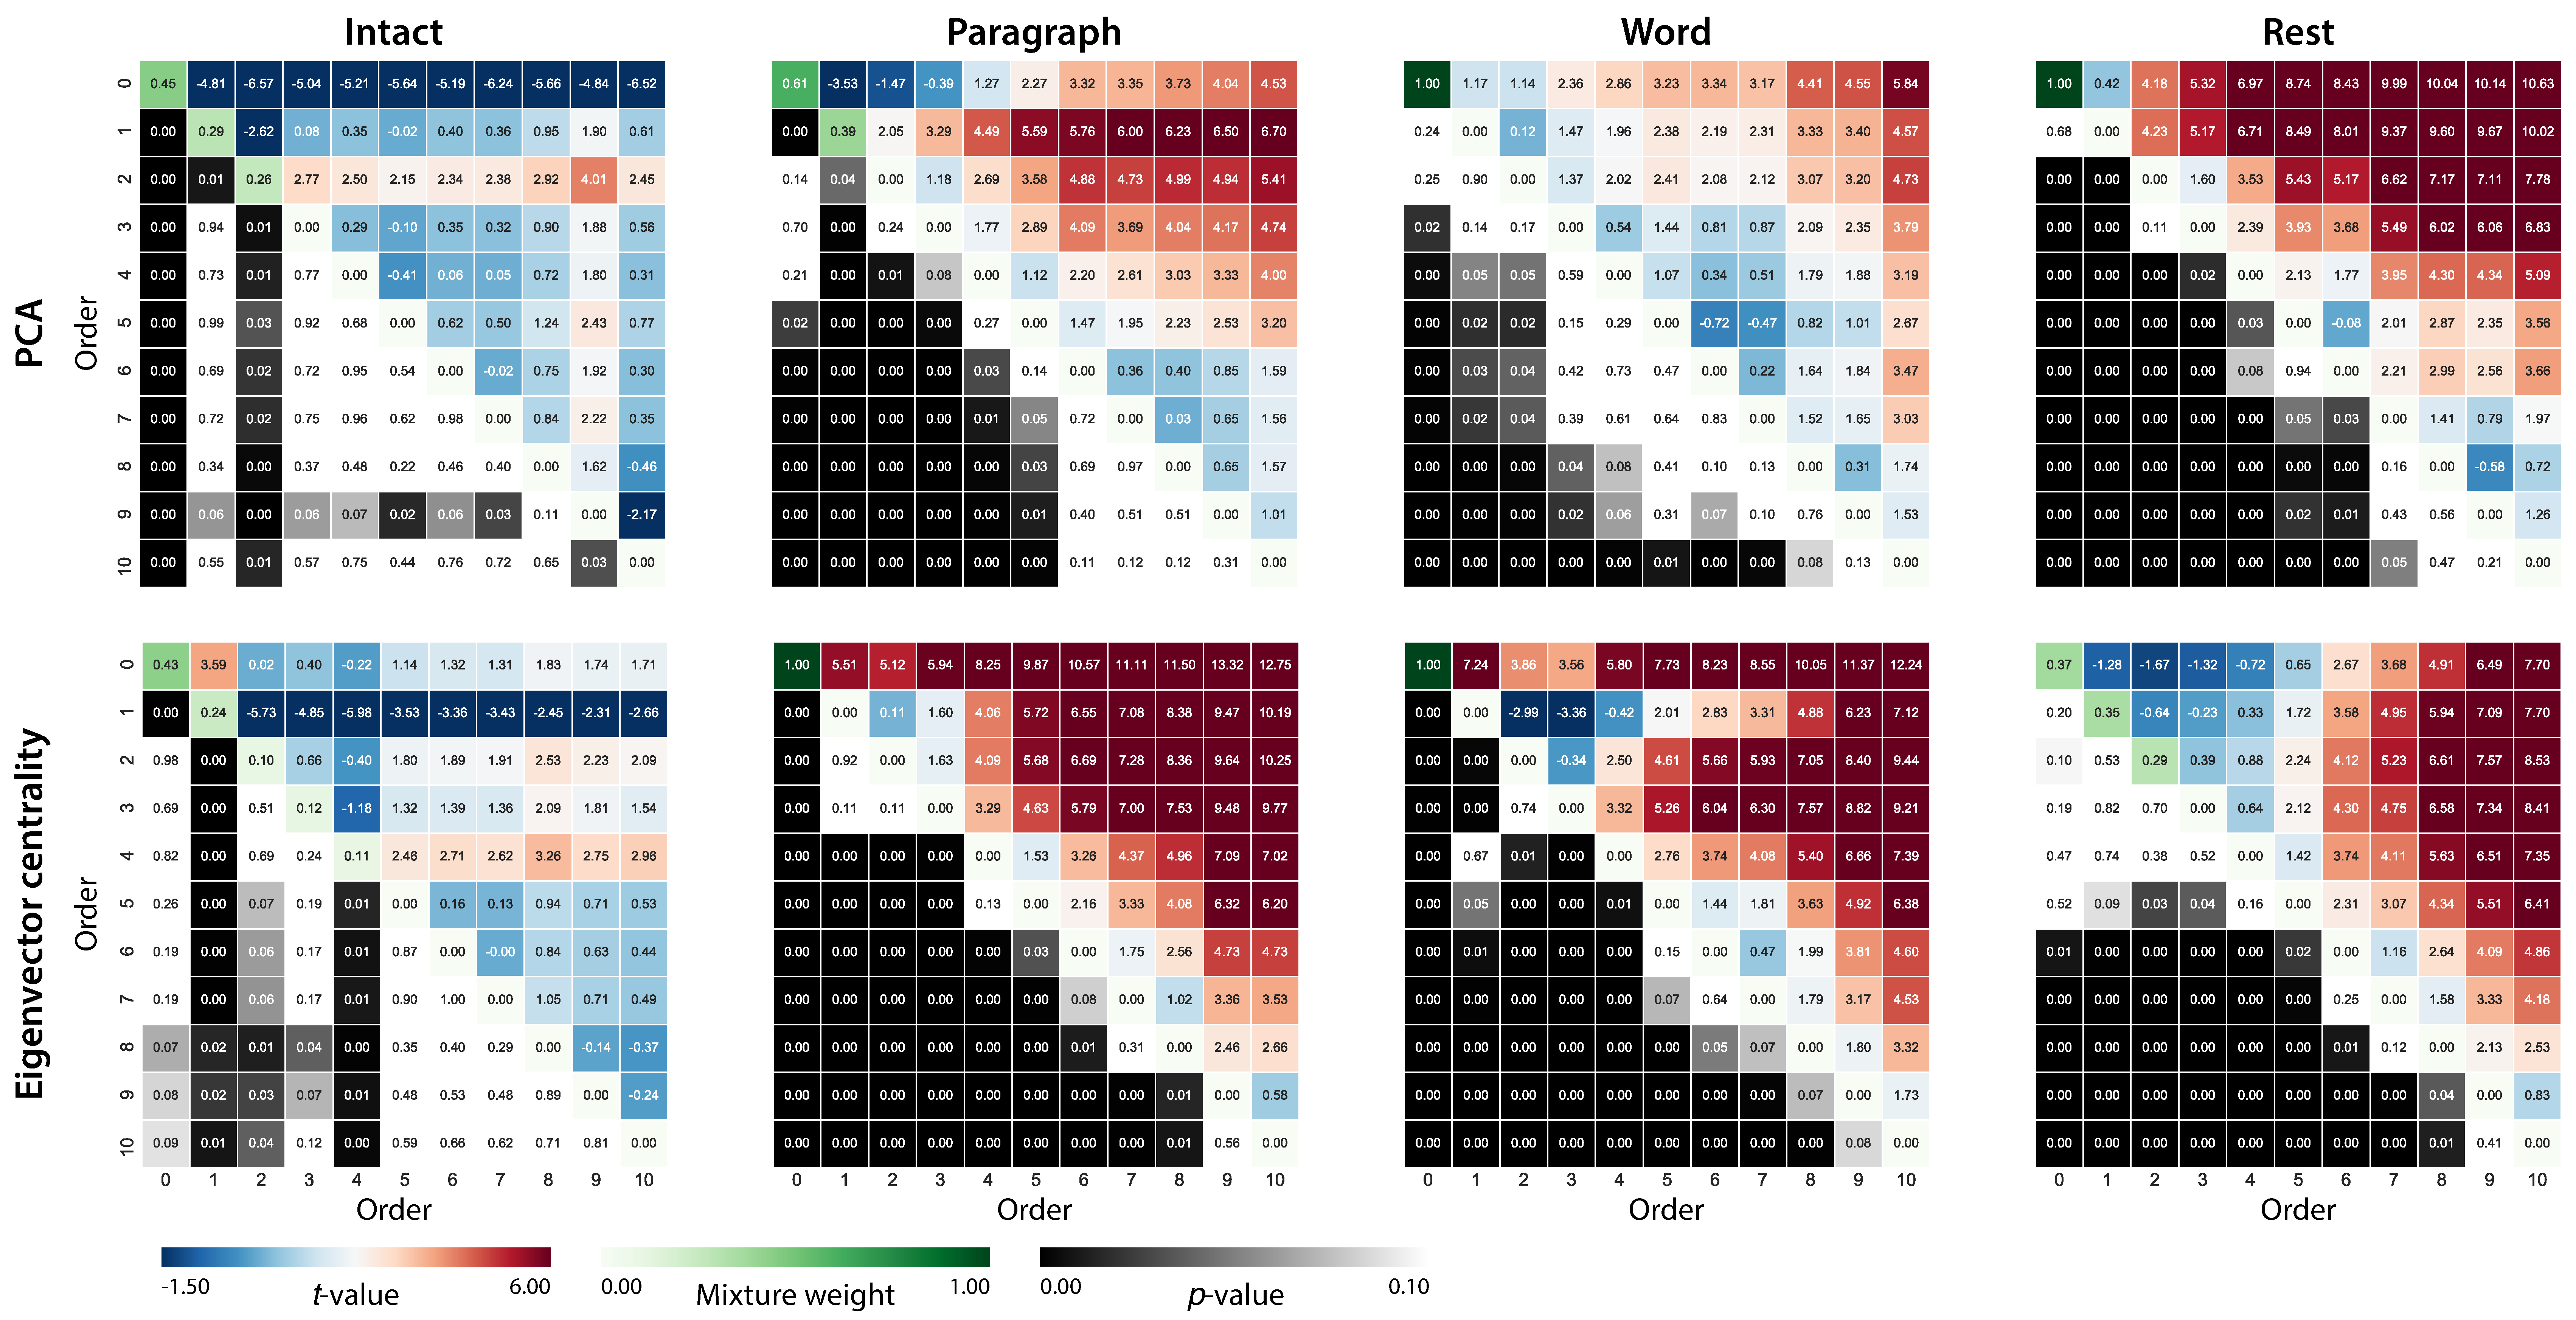
\includegraphics[width=1\textwidth]{figs/stats_heatmaps}
\caption{\textbf{Statistical summary of decoding accuracies for
    different neural features.}  Each column displays decoding
  results for one experimental condition (intact, paragraph, word, and
  rest).  We considered dynamic activity patterns (order 0) and
  dynamic correlations at different orders (order $> 0$).  We used
  two-tailed $t$-tests to compare the
  distributions of decoding accuracies obtained using each pair of
  features.  The distributions for each feature reflect the set of
  average decoding accuracies (across all kernel parameters), obtained
  for each random assignment of training and test groups.
  In the upper triangles of each map, warmer colors (positive $t$-values) indicate that the
  neural feature indicated in the given row yielded higher accuracy than the
  feature indicated in the given column.  Cooler colors (negative
  $t$-values) indicate that
  the feature in the given row yielded lower decoding accuracy than
  the feature in the given column.  The lower triangles of each map
  denote the corresponding $p$-values for the $t$-tests.  The diagonal
  entries display the relative average optimized weight given to each type of feature, in
  a decoder that included all feature types (see \textit{Feature
    weighting and testing}).}
\label{fig:ttests}
\end{figure}

Both sets of temporal decoding analyses yielded qualitatively similar
results for the auditory (non-rest) conditions of the experiment
(Fig.~\ref{fig:decoding}: pink, yellow, and teal lines;
Fig.~\ref{fig:ttests}: three leftmost columns).  The highest
decoding accuracy for participants who listened to the intact
(unscrambled) story was achieved using high-order dynamic correlations
(PCA: second-order; eigenvector-centrality: fourth-order).  Scrambled
versions of the story were best decoded by lower-order correlations
(PCA/paragraph: first-order; PCA/word: order zero; eigenvector
centrality/paragraph: order zero; eigenvector centrality/word: order
zero).  The two sets of analyses yielded different decoding results on
resting state data (Fig.~\ref{fig:decoding}: purple lines;
Fig.~\ref{fig:ttests}: rightmost column).  We note
that while the resting state times could be decoded reliably, the
accuracies were only very slightly above chance.  We speculate that
the decoders might have picked up on attentional drift, boredom, or
tiredness; we hypothesize that these all increased throughout the resting
state scan.  The decoders might be picking up on aspects of these
loosely defined cognitive states that are common across individuals.
The PCA-based approach achieved the highest resting state decoding
accuracy using order zero features (non-correlational,
activation-based), whereas the eigenvector centrality-based approach
achieved the highest resting state decoding accuracy using
second-order correlations.  Taken together, these analyses indicate
that high-level cognitive processing (while listening to the intact
story) is reflected in the dynamics of high-order correlations in
brain activity, whereas lower-level cognitive processing (while
listening to scrambled versions of the story that lack rich meaning)
is reflected in the dynamics of lower-order correlations and
non-correlational activity dynamics.  Further, these patterns are
associated both with the underlying activity patterns (characterized
using PCA) and also with the changing relative positions that
different brain areas occupy in their associated networks
(characterized using eigenvector centrality).

\begin{figure}[tp]
  \centering
  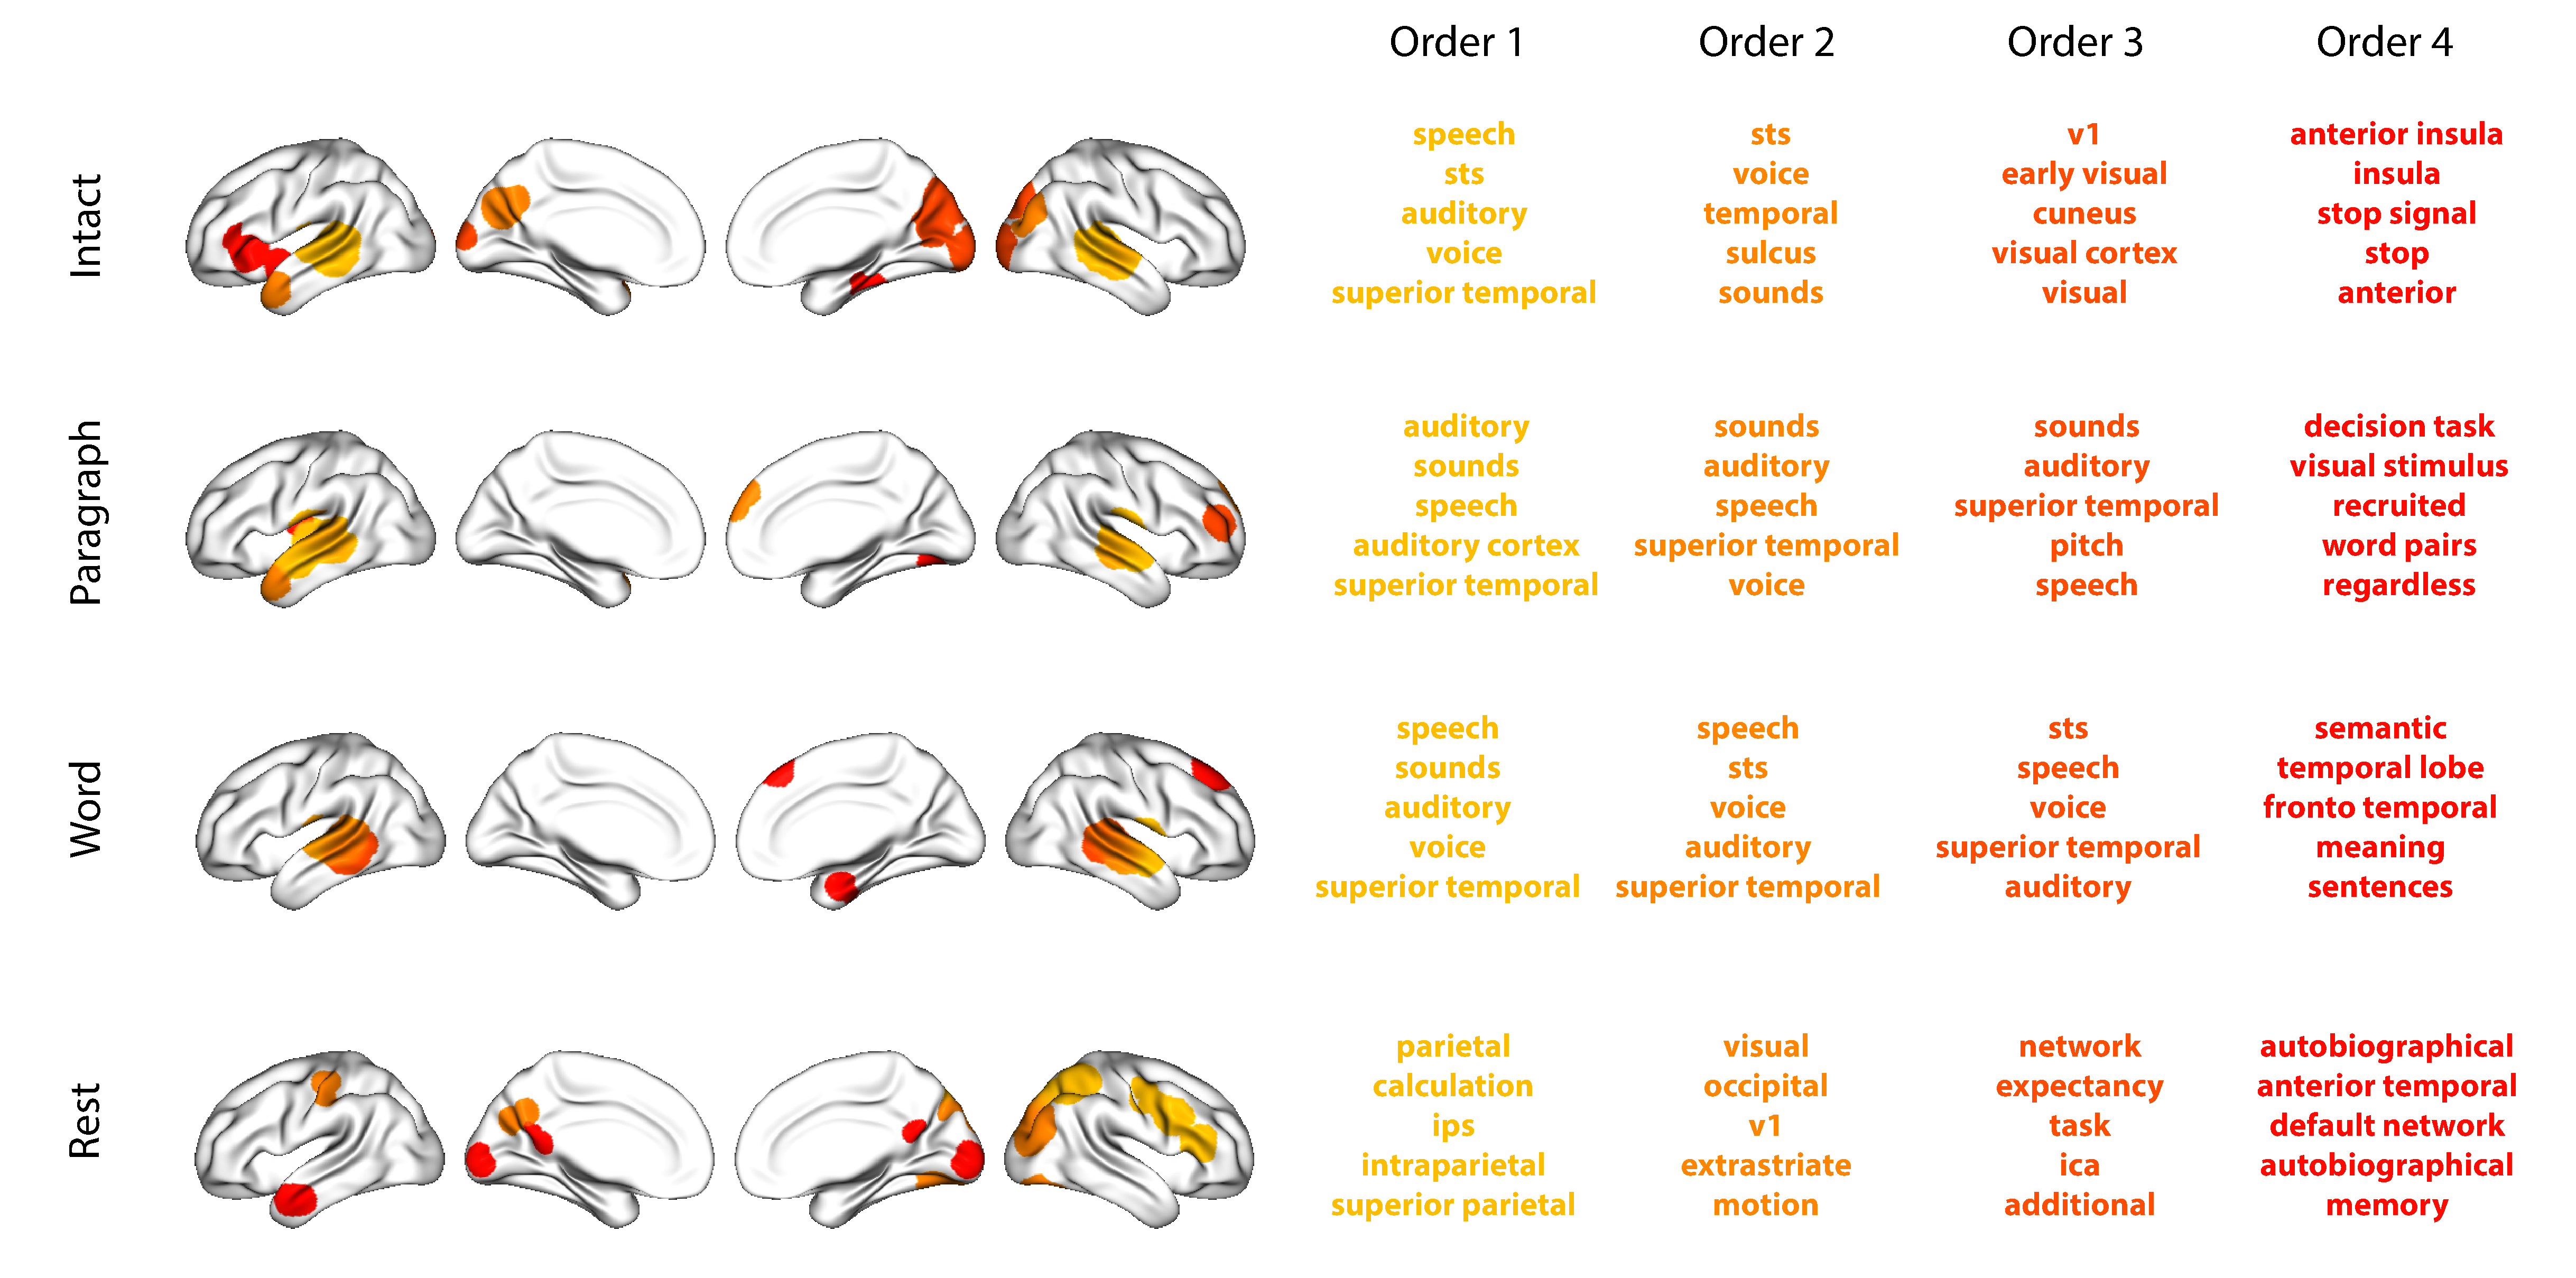
\includegraphics[width=\textwidth]{figs/most_abs}
  \caption{\textbf{Top terms associated with the endpoints of the
      strongest correlations.}  Each color corresponds to one order of
    inter-subject functional correlations. The inflated brain plots
    display the locations of the endpoints of the 10 strongest
    (absolute value) correlations at each order, projected onto the
    cortical surface~\citep{CombEtal19}.  The lists of terms on the
    right display the top five Neurosynth terms~\citep{RubiEtal17}
    decoded from the corresponding brain maps for each order.  Each
    row displays data from a different experimental condition.
    Additional maps and their corresponding Neurosynth terms may be
    found in the \textit{Supplementary materials} (intact: Figure~\intact;
    paragraph: Figure~\para; word: Figure~\word; rest: Figure~\rest).}
  \label{fig:neurosynth}
\end{figure}

Having established that patterns of high-order correlations are
informative to decoders, we next wondered which specific networks of
brain regions contributed most to these patterns.  As a representative
example, we selected the kernel parameters that yielded decoding
accuracies that best matched the average accuracies across all of the
kernel parameters we examined.  Using Figure~\ref{fig:decoding}c as a
template, the best-matching kernel was a Laplace kernel with a width
of 50 (Fig.~\ref{fig:kernels}d).  We used this kernel to compute a
single $K$ by $K$ $n^\mathrm{th}$-order DISFC matrix for each
experimental condition.  We then used Neurosynth~\citep{RubiEtal17} to
compute the terms most highly associated with the most strongly
correlated pairs of regions in each of these matrices
(Fig.~\ref{fig:neurosynth}; see \textit{Reverse inference}).

For all of the story listening conditions (intact, paragraph, and
word), we found that first- and second-order correlations were most
strongly associated with auditory and speech processing areas.  During
intact story listening, third-order correlations reflected integration
with visual areas, and fourth-order correlations reflected integration
with areas associated with high-level cognition and cognitive control,
such as the ventrolateral prefrontal cortex.  However, during
listening to temporally scrambled stories, these higher-order
correlations instead involved interactions with additional regions
associated with speech and semantic processing.  By contrast, we found
a much different set of patterns in the resting state data.
First-order resting state correlations were most strongly associated
with regions involved in counting and numerical understanding.
Second-order resting state correlations were strongest in visual
areas; third-order correlations were strongest in task-positive areas;
and fourth-order correlations were strongest in regions associated
with autobiographical and episodic memory.  We carried out analogous
analyses to create maps (and decode the top associated Neurosynth
terms) for up to fifteenth-order correlations (Figs.~\intact, \para, \word, and
\rest).  Of note, examining fifteenth-order correlations between 700
nodes using conventional methods would have required storing roughly
$\frac{700^{2 \times 15}}{2} \approx 1.13 \times 10^{85}$ floating
point numbers-- assuming single-precision (32 bits each), this would
require roughly 32 times as many bits as there are molecules in the
known universe!  Although these fifteenth-order correlations do appear
(visually) to have some well-formed structure, we provide this latter
example primarily as a demonstration of the efficiency and scalability
of our approach.






%%%%%%%%%%%%%%%%%%%%%%%%%%%%%%%%%%%%%%%
\section*{Discussion}
We tested the hypothesis that high-level cognition is supported by
high-order brain network dynamics~\citep[e.g., see][]{SoloEtal19,
  ReimEtal17}.  We examined high-order network dynamics in functional
neuroimaging data collected during a story listening experiment.  When
participants listened to an auditory recording of the story,
participants exhibited similar high-order brain network dynamics.  By
contrast, when participants instead listened to temporally scrambled
recordings of the story, only lower-order brain network dynamics were
similar across participants.  Our results indicate that higher orders
of network interactions support higher-level aspects of cognitive
processing (Fig.~\ref{fig:discussion}).

\begin{figure}[tp]
  \centering
  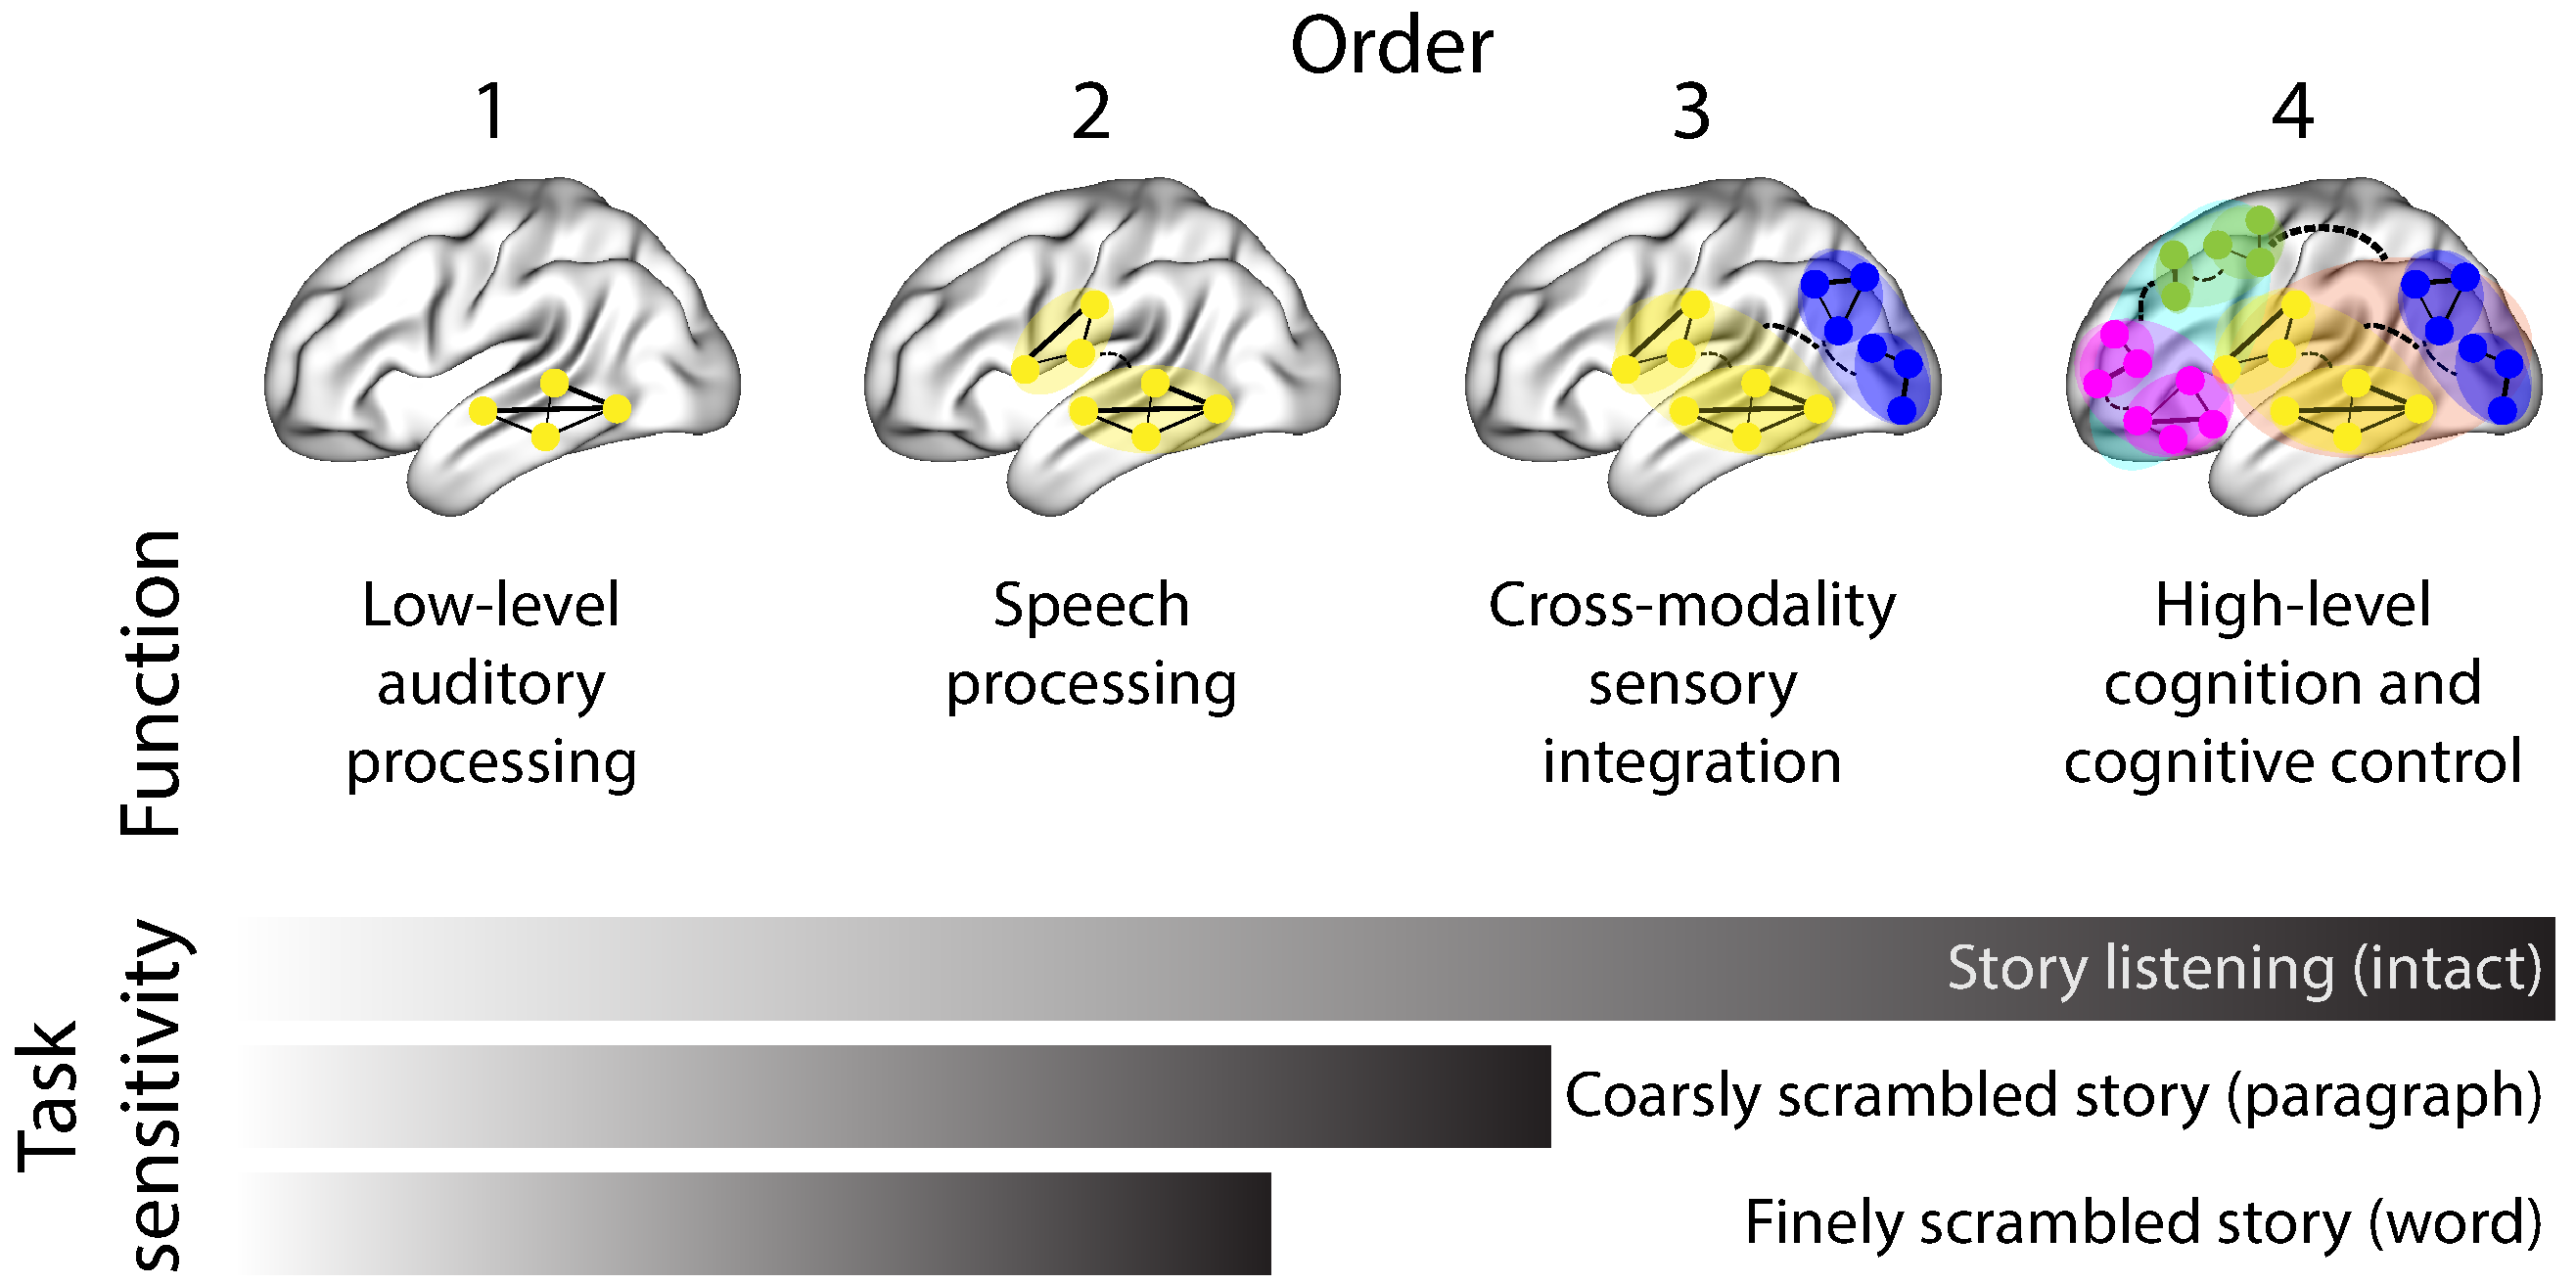
\includegraphics[width=0.6\textwidth]{figs/discussion}
  \caption{\textbf{Proposed high-order network dynamics underlying
      high-level cognition during story listening.}  Higher orders of
    network interactions support higher-level aspects of cognitive
    processing.  When tasks evoke richer, deeper, and/or higher-level
    processing, this is reflected in higher-order network
    interactions.}
  \label{fig:discussion}
\end{figure}

The notion that cognition is reflected in (and possibly mediated by)
patterns of first-order network dynamics has been suggested by or
proposed in myriad empirical studies and
reviews~\citep[e.g.,][]{DemeEtal19, Turk13, LuriEtal18, FongEtal19,
  ParkEtal18b, PretEtal17, RoyEtal19, LiegEtal19, ZouEtal19,
  ChanGlov10, GonzEtal19}.  Our study extends this line of work by
finding cognitively relevant \textit{higher-order} network dynamics
that reflect ongoing cognition.  Our findings complement other work
that uses graph theory and topology to characterize how brain networks
reconfigure during cognition~\citep[e.g.,][]{BassEtal06, ZhenEtal19,
  McInJirs19, TokeSomm19, SizeEtal18, ReimEtal17, BetzEtal19}.

An open question not addressed by our study pertains to how different
structures integrate incoming information with different time
constants.  For example, one line of work suggests that the cortical
surface comprises a structured map such that nearby brain structures
process incoming information at similar timescales.  Low-level sensory
areas integrate information relatively quickly, whereas higher-level
regions integrate information relatively slowly~\citep{BaldEtal17,
  HassEtal08, HassEtal15, HoneEtal12a, LernEtal11, LernEtal14}.  Other
related work in human and mouse brains indicates that the temporal
response profile of a given brain structure may relate to how strongly
connected that structure is with other brain
areas~\citep{FallEtal19}.  Further study is needed to understand the
role of temporal integration at different scales of network
interaction, and across different anatomical structures.

Another potential limitation of our approach relates to recent work
suggesting that the brain undergoes rapid state changes, for example
across event boundaries~\citep[e.g.,][]{BaldEtal17}.
\cite{ShapEtal19} used hidden semi-Markov models to estimate
state-specific network dynamics~\citep[also see][]{VidaEtal18}.  Our
general approach might be extended by considering putative state
transitions. For example, rather than weighting all timepoints using a
similar kernel (Eqn.~\ref{eqn:timecorr}), the kernel function could
adapt on a timepoint-by-timepoint basis such that only timepoints
determined to be in the same ``state'' were given non-zero weight.

Identifying higher-order network dynamics associated with high-level
cognition required several important methods advances.  First, we used
kernel-based dynamic correlations to extended the notion of (static)
inter-subject functional connectivity~\citep{SimoEtal16} to a dynamic
measure of inter-subject functional connectivity (DISFC) that does not
rely on sliding windows, and that may be computed at individual
timepoints.  This allowed us to precisely characterize stimulus-evoked
network dynamics that were similar across individuals.  Second, we
developed a computational framework for efficiently and scalably estimating
high-order dynamic correlations.  Our approach uses dimensionality
reduction algorithms and graph measures to obtain low-dimensional
embeddings of patterns of network dynamics.  Third, we developed an
analysis framework for identifying robust decoding results by carrying
out our analyses using a range of parameter values and then
identifying which results were robust to specific parameter choices.

\subsection*{Concluding remarks}
The complex hierarchy of dynamic interactions that underlie our
thoughts is perhaps the greatest mystery in modern science.  Methods
for characterizing the dynamics of high-order correlations in neural
data provide a window into the neural basis of cognition.  By showing
that high-level cognition is reflected in high-order network dynamics,
we have elucidated the next step on the path towards understanding the
neural basis of cognition.


\section*{Acknowledgements}
We acknowledge discussions with Luke Chang, Vassiki Chauhan, Hany
Farid, Paxton Fitzpatrick, Andrew Heusser, Eshin Jolly, Aaron Lee,
Qiang Liu, Matthijs van der Meer, Judith Mildner, Gina Notaro, Stephen
Satterthwaite, Emily Whitaker, Weizhen Xie, and Kirsten Ziman. Our
work was supported in part by NSF EPSCoR Award Number 1632738 to
J.R.M. and by a sub-award of DARPA RAM Cooperative Agreement
N66001-14-2-4-032 to J.R.M.  The content is solely the responsibility
of the authors and does not necessarily represent the official views
of our supporting organizations.

\section*{Author contributions}
Concept: J.R.M.  Implementation: T.H.C., L.L.W.O., and J.R.M.
Analyses: L.L.W.O. and J.R.M.  Writing: L.L.W.O. and J.R.M.

\bibliographystyle{apacite}
\bibliography{CDL-bibliography/memlab}

\end{document}


